\documentclass[12pt]{article}
% \usepackage{subfigure}
\usepackage{graphicx}
%in that file you will find the packages and other macro needed like \R for the real number set. 
\usepackage{vmargin}
\setmarginsrb{28mm}{25mm}{28mm}{25mm}{0pt}{0mm}{0pt}{0mm}
\setlength{\footskip}{20pt}
\usepackage{amssymb}
\usepackage{amsmath}
\usepackage{amsthm}
\usepackage{pgfplots} 
\usepackage{graphicx}
\usepackage[utf8x]{inputenc}
\usepackage{tikz}
\usepackage{bbm}
\usepackage{subcaption}
\usepackage[boxruled]{algorithm2e}
\usepackage{mathtools}
\usepackage{lipsum}
\usepackage[title,titletoc]{appendix}
\usepackage{booktabs}
\usepackage{here}
\usepackage[]{hyperref}
\usepackage{natbib,enumerate} 

%some weird packages
\usepackage{halloweenmath}
\usepackage{txfonts}
\usepackage{knitting}

\DeclarePairedDelimiter{\ceil}{\lceil}{\rceil}
\renewcommand{\phi}{\varphi}
\newcommand{\eqtext}[1]{\ensuremath{\stackrel{#1}{=}}}
\newcommand{\leqtext}[1]{\ensuremath{\stackrel{#1}{\leq}}}
\newtheorem{theorem}{Proposition}[section]
\newtheorem{lemma}{Lemma}[section]
\newtheorem{remark}{Remark}[section]
\newcommand{\N}{\mathbb{N}}
\newcommand{\R}{\mathbb{R}}
\newcommand{\E}{\mathbb{E}}
\newcommand{\epl}{\varepsilon}


\date{\today}

\begin{document}

%this creates the title page. You must complete the information therehttps://cn.overleaf.com/project/627e20a1da1b6135dd2e88af
\begin{titlepage}
    \newcommand{\HRule}{\rule{\linewidth}{0.5mm}} % Defines a new command for the horizontal lines, change thickness here
    
    \center % Center everything on the page
     
    %----------------------------------------------------------------------------------------
    %   HEADING SECTIONS
    %----------------------------------------------------------------------------------------
    
    \vspace{3cm}
    \textsc{\LARGE École polytechnique fédérale de Lausanne}\\[1.5cm] % Name of your university/college
    \textsc{\Large Semester project}\\[0.5cm] % Major heading such as course name
    \textsc{\large Master in Computational science and Engineering}\\[0.5cm] % Minor heading such as course title
    
    %----------------------------------------------------------------------------------------
    %   TITLE SECTION
    %----------------------------------------------------------------------------------------
    
    \HRule \\[0.4cm] % line above and under the title
    { \huge \bfseries Automatic vectorization of the  \\ renovated cadastre of Lausanne}\\[0.4cm] % Title of your document
    \HRule \\[1.5cm]
     
    %----------------------------------------------------------------------------------------
    %   AUTHOR SECTION
    %----------------------------------------------------------------------------------------
    
    \begin{minipage}{0.4\textwidth}
    \begin{flushleft} \large
    \emph{Author:}\\
    Danyang \textsc{Wang} % Your name
    \end{flushleft}
    \end{minipage}
    ~
    \begin{minipage}{0.4\textwidth}
    \begin{flushright} \large
    \emph{Supervisor:} \\
    Rémi \textsc{Guillaume Petitpierre}
    Frederic \textsc{Kaplan} % Supervisor's Name
    \end{flushright}
    \end{minipage}\\[10cm]
    
    %----------------------------------------------------------------------------------------
    %   LOGO SECTION
    %----------------------------------------------------------------------------------------
    
    
\includegraphics[width=0.4\linewidth]{Logo}\\[1cm] % Include a department/university logo - this will require the graphicx package
     
    %----------------------------------------------------------------------------------------
    
    \vfill % Fill the rest of the page with whitespace
    
    \end{titlepage}
    

\clearpage
\thispagestyle{empty}
\tableofcontents

\clearpage
\pagenumbering{arabic}
\setcounter{page}{1}

\section{Introduction}
Historical cadastral maps are an indispensable source for studying the evolution of our cities. We have a "renovated cadastre" which consists of more than 300 plates with high quality and accuracy and two copies are well-preserved today and have been well-scanned. Transforming these cadastres into vector maps can help researchers better utilize them with higher efficiency and also prevent these precious historical documents from being damaged and lost. In this automatic vectorization project, we found a method to transform those well-scanned historical cadastre maps into polygon-segmented images with automatic computer vision methods.

We first present semantic segmentation with a convolutional neural network (CNN) model to detect all the edges and boundaries of objects in these cadastres, and then we use the computer vision method to recover all the polygons by segmenting regions from the CNN prediction outputs and finally get polygon-segmented images. In the future researchers can utilize these polygon recovery results and transform them into vector images by just manual labeling with particular software.

\section{Data annotation}

\subsection{Dataset}
The renovated cadastre was measured and drawn by Deluz in 1888, which consists of more than 300 historical maps of Lausanne with similar scale ratios from 1:500 to 1:2000. We decided to use 24 of these cadastre maps to explore automatic methods for image vectorization. 13 of the maps have a scale comprised of 1:500 and 9 maps with a scale ratio of 1:1000 and the remaining 2 maps with a scale ratio of 1:2000. An example of the cadastre is shown in Figure \ref{fig:cadaster-preprocessing} (a), which depicted a region of city of historical Lausanne.   
\begin{figure}[H]
	\begin{subfigure}[b]{.66\textwidth}
		% include first image
		\centering
		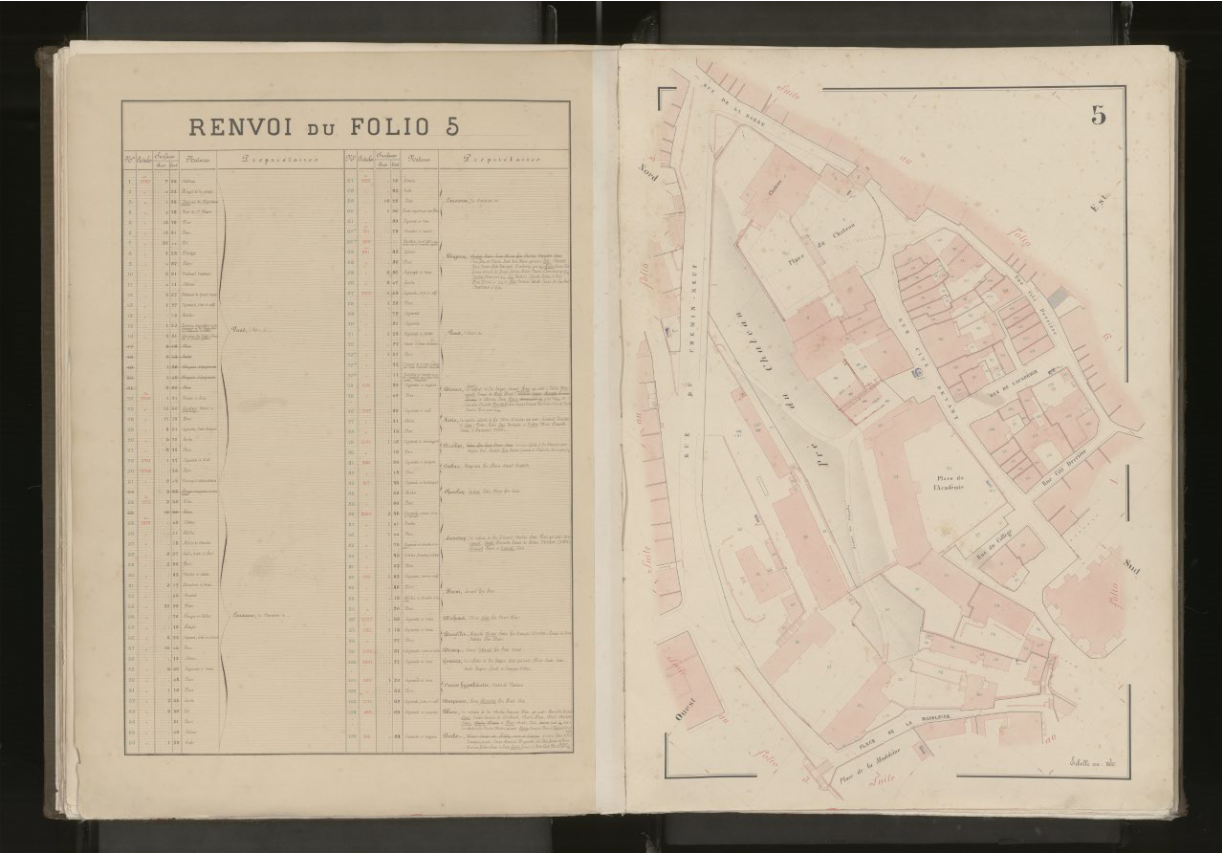
\includegraphics[height=200pt]{images/original.jpg}  
		\label{fig:original-images}
		\caption{Example of original cadastre}
	\end{subfigure}
	\begin{subfigure}[b]{.33\textwidth}
		% include second image
		\centering
		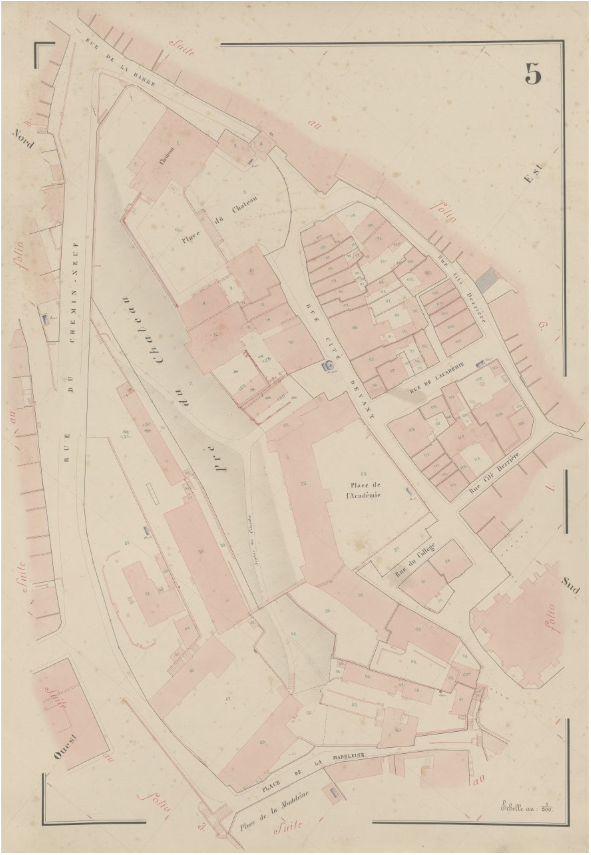
\includegraphics[height=200pt]{images/img1.png}  
		\label{fig:cropped-images}
		\caption{cropped map}
	\end{subfigure}
	
	\caption{Cadastre preprocessing}
	\label{fig:cadaster-preprocessing}
\end{figure}

We found that, all of those scanned cadastre pages consist of map images in the right parts, and the left parts are just some text descriptions and forms that are not interested in this map processing project, and there are also black backgrounds at the boundary of these cadastre images. so we can just retain the map part and cut out the black edges and the left part of these cadastre images. Figure \ref{fig:cadaster-preprocessing} (b) showed the map image after cropping, and our project was carried out based on those cropped maps. 
\subsection{Annotation}

Every cadastre map described road networks, buildings, rivers, fountains, and other cartographic contents of part of the Lausanne. We call those map elements mentioned above "edge", and the aim of the data annotation is to label all the "edges" in each cadastre map and generate a binary edge image for each map for model training in the semantic segmentation process.
 
Since annotation is a greatly boring and time-consuming work since we need to judge every detail of the map and annotate with very high accuracy and also considering the limited time and human resources, we selected 12 of those 24 maps to make the annotation work, containing 3 of them described part of the urban area of Lausanne with a high density of buildings and road networks, 6 of them shows part of countryside regions, and the last 3 maps contain just some rivers and roads with very few buildings.

The annotation process was done with a raster-based software called "GNU Image Manipulation Program". We annotated class "edge" with 6-pixels-wide lines. Figure \ref{fig:anno_res} shows the patches of original maps and their corresponding annotation results. We can see that these maps consist of different colors of lines. Black lines (solid and dotted) (Figure \ref{fig:anno_res} 2. (a)) are road networks, red lines are building edges and walls and other human-made barriers, and a few blue lines exist which are railway networks (Figure \ref{fig:anno_res} 1. (c)). 



\begin{figure}[H]
    \centering
    \rotatebox{90}{\scriptsize{~~~~~~~~~~~~~~~~~~1. Image}}
    \begin{subfigure}[b]{.235\textwidth}
		\begin{minipage}[t]{1\linewidth}
			\centering
			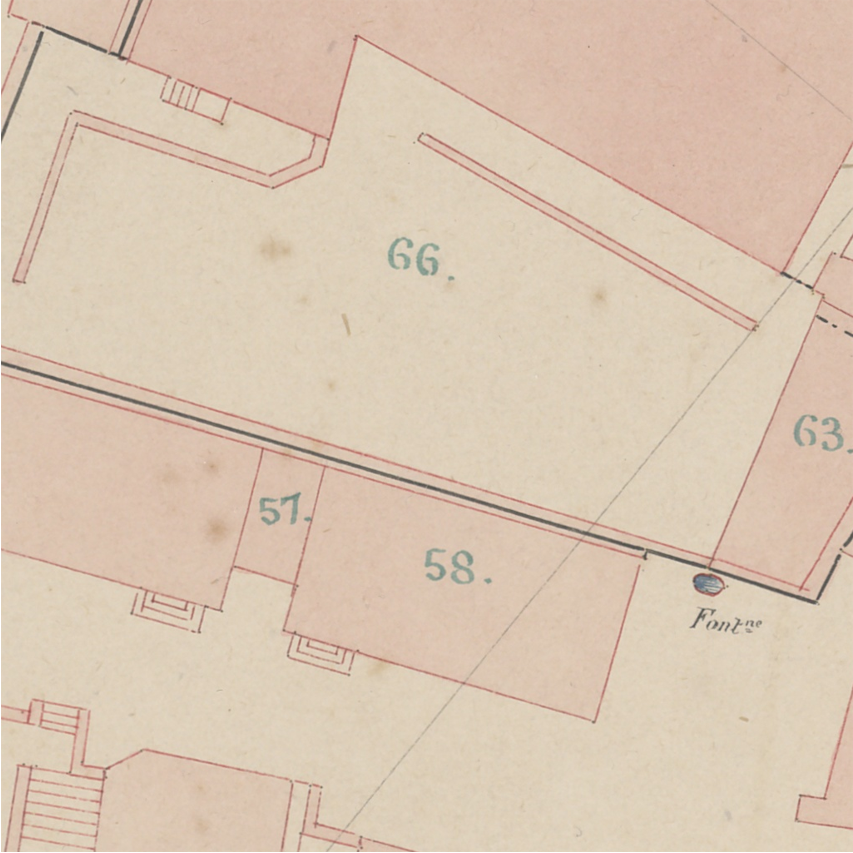
\includegraphics[width=1\linewidth]{images/patches/img1.png}
		\end{minipage}
	\end{subfigure}
	\begin{subfigure}[b]{.235\textwidth}
		\begin{minipage}[t]{1\linewidth}
			\centering
			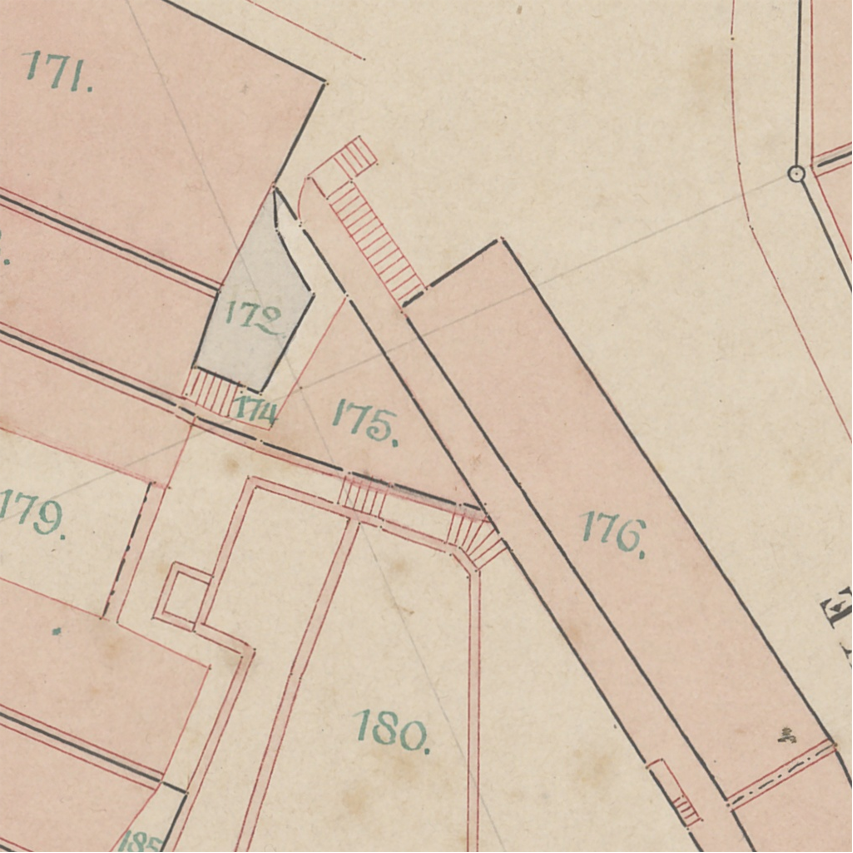
\includegraphics[width=1\linewidth]{images/patches/img4.png}
		\end{minipage}
	\end{subfigure}
	\begin{subfigure}[b]{.235\textwidth}
		\begin{minipage}[t]{1\linewidth}
			\centering
			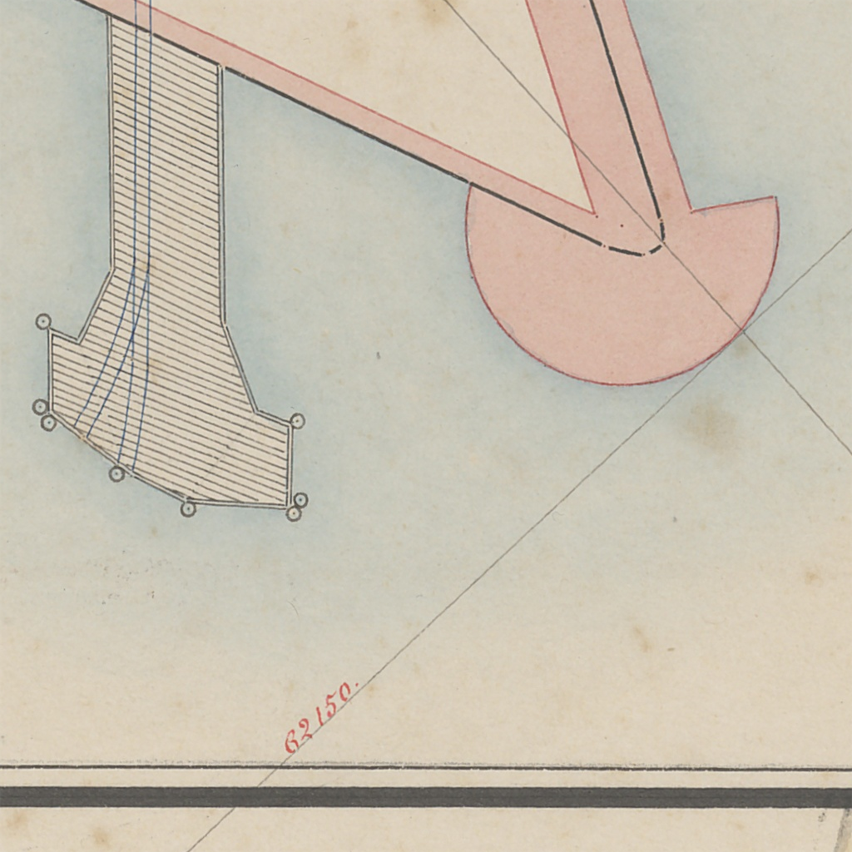
\includegraphics[width=1\linewidth]{images/patches/img8.png}
		\end{minipage}
	\end{subfigure}
	\begin{subfigure}[b]{.235\textwidth}
		\begin{minipage}[t]{1\linewidth}
			\centering
			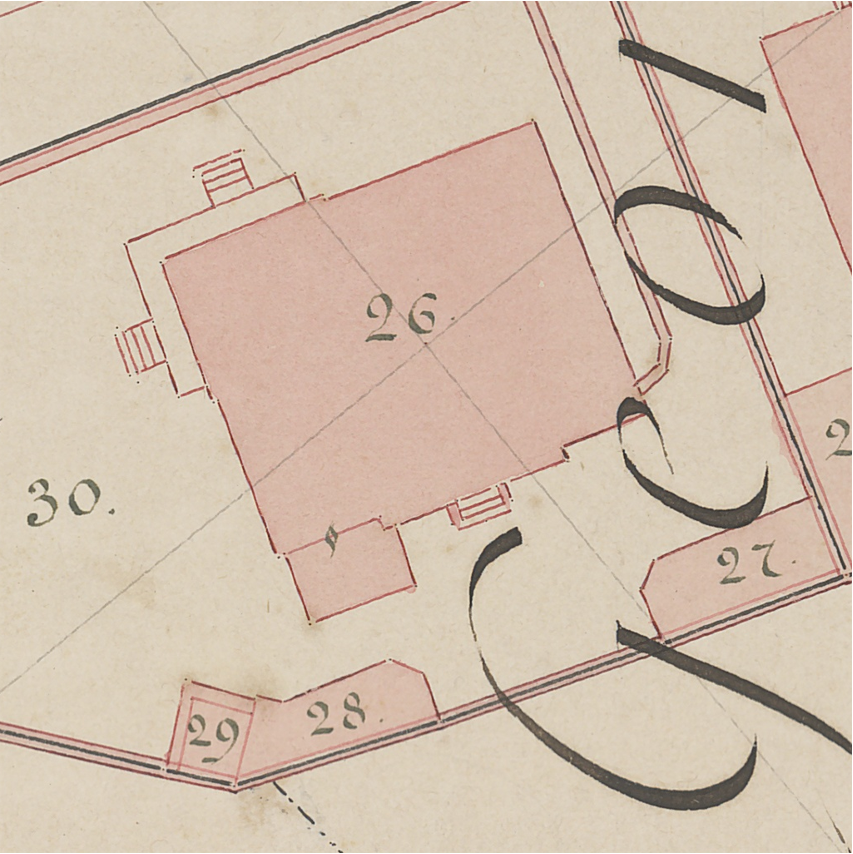
\includegraphics[width=1\linewidth]{images/patches/img7.png}
		\end{minipage}
	\end{subfigure}
	
 `
    % 两行图片的间隙有点大,通过vspace进行微调
	\vspace{-3mm}
    % 由于上面已经用了subfigure,下面我们希望从 a 重新编号,而不是从 d 开始,清零。
	\setcounter{subfigure}{0}
	
 
    % 第二行图片展示
    \rotatebox{90}{\scriptsize{~~~~~~~~~2. Annotation result}}
    \begin{subfigure}[b]{.235\textwidth}
        % 左标题2
		
		\begin{minipage}[t]{1\linewidth}
			\centering
			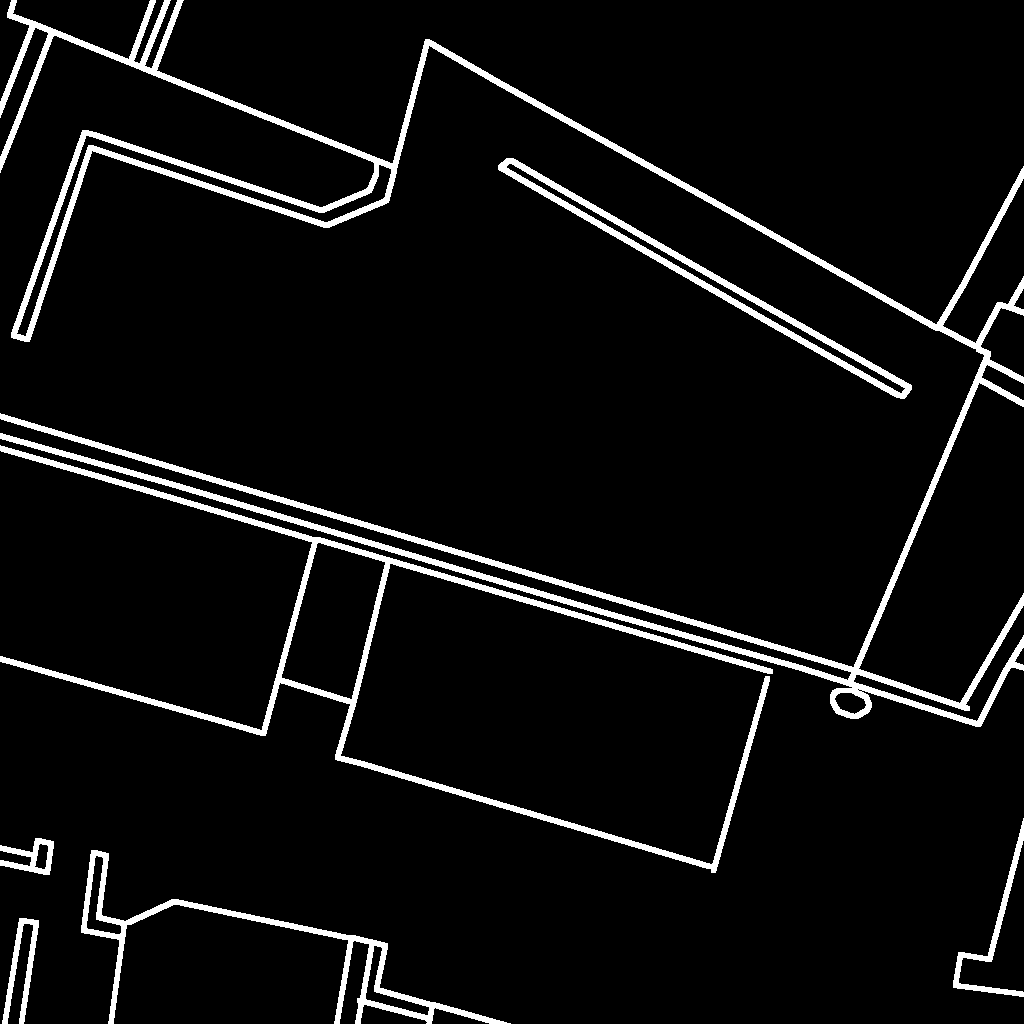
\includegraphics[width=1\linewidth]{images/patches/gt1.png}
			\caption{ }
		\end{minipage}
	\end{subfigure}
	\begin{subfigure}[b]{.235\textwidth}
		\begin{minipage}[t]{1\linewidth}
			\centering
			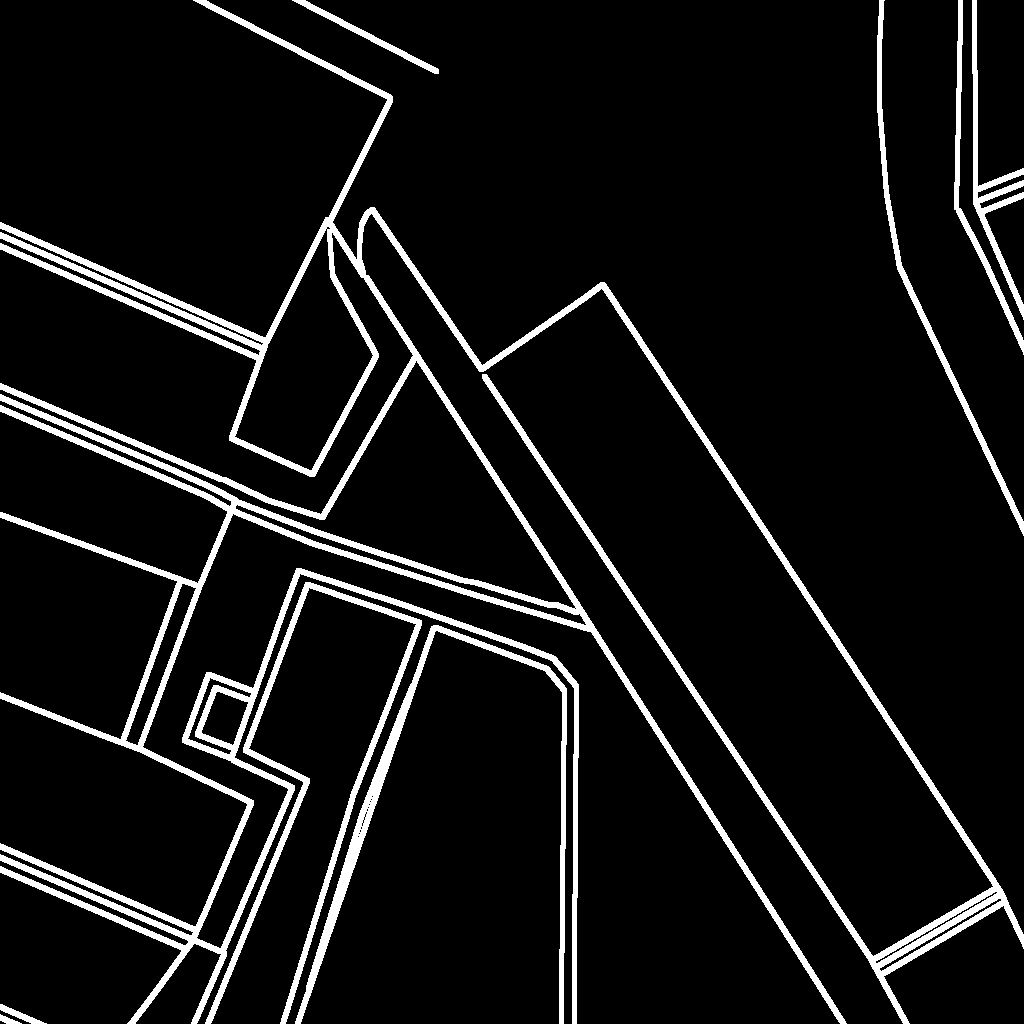
\includegraphics[width=1\linewidth]{images/patches/gt4.png}
			\caption{ }
		\end{minipage}
	\end{subfigure}
	\begin{subfigure}[b]{.235\textwidth}
		\begin{minipage}[t]{1\linewidth}
			\centering
			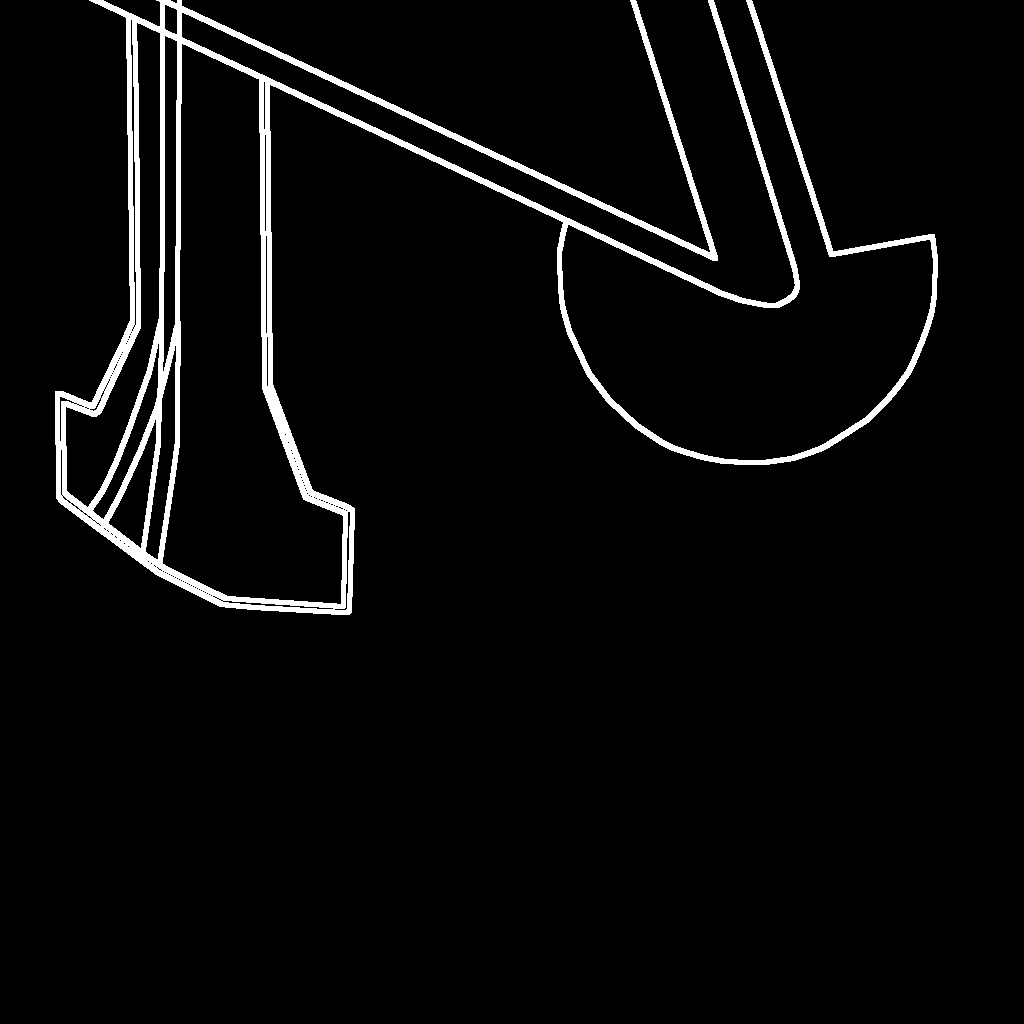
\includegraphics[width=1\linewidth]{images/patches/gt8.png}
		    \caption{ }
		\end{minipage}
	\end{subfigure}
	\begin{subfigure}[b]{.235\textwidth}
		\begin{minipage}[t]{1\linewidth}
			\centering
			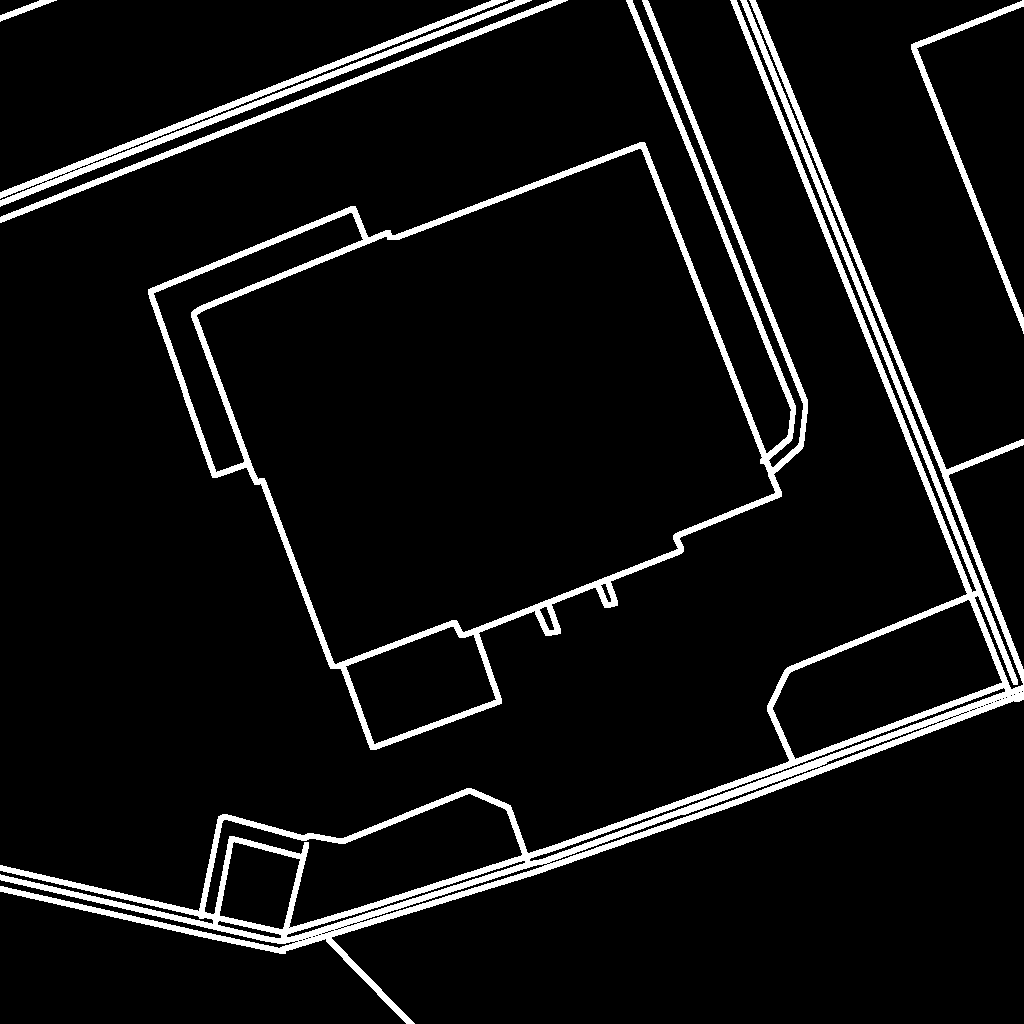
\includegraphics[width=1\linewidth]{images/patches/gt7.png}
		    \caption{ }
		\end{minipage}
	\end{subfigure}
	
    \caption{Patches if annotation results}
    \label{fig:anno_res}
\end{figure}

We should notice that there are also some perpendicular thin straight lines throughout the whole map, which are just geometrical lines that were not interested thus we should not annotate them, and some text descriptions are contained in these maps (Figure \ref{fig:anno_res} 1. (d)) and some of them are even overlapped with road networks and buildings and thus could bring difficulty in annotating and result in prediction error in the semantic segmentation task, and we should keep labeling straight lines and ignore these texts during annotation (Figure \ref{fig:anno_res} 2. (d)). There are also some stairs near or in the buildings with some dense parallel lines and considering that annotating them will split a lot of little polygons which is not needed in the polygon recovery task, we decided to ignore those stairs during annotation (Figure \ref{fig:anno_res} 1-2. (b)).

Figure \ref{fig:whole-annotation} shows an example of the original maps and their corresponding annotation results. All the white lines are the "edge" class and the remaining black domains are "background". The total annotation task took about 5 weeks of work with a 1.5 day/week workload.

\begin{figure}[H]
    
	\begin{subfigure}[b]{0.5\textwidth}
		% include first image
	    \centering
		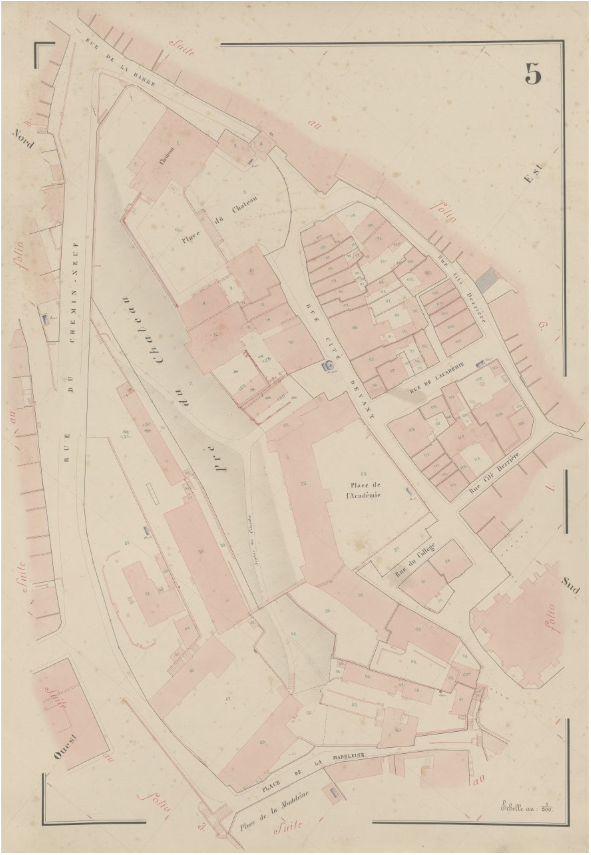
\includegraphics[width=1\linewidth]{images/img1.png}  
		\label{fig:}
	\end{subfigure}
	\begin{subfigure}[b]{.5\textwidth}
		% include second image
		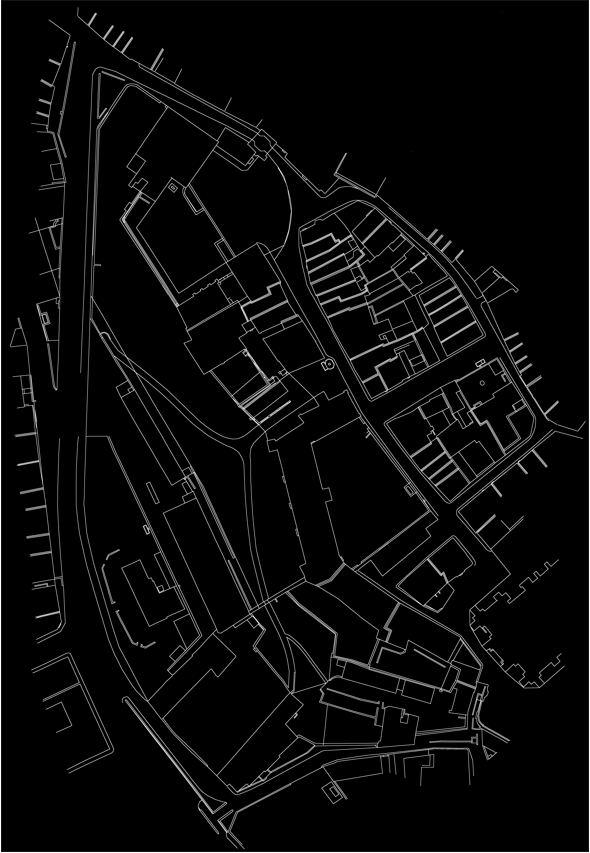
\includegraphics[width=1\linewidth]{images/label1.png}  
		\label{fig:sub-second}
	\end{subfigure}
	
	\caption{Original maps and their annotation results}
	\label{fig:whole-annotation}
\end{figure}



\section{Semantic segmentation}
Convolutional neural networks (CNNs)  have shown impressive performance for image segmentation tasks  (i.e.,  to determine whether a pixel belongs to a certain object or not)\cite{heitzler2020cartographic}. Dataset consists of input images (original maps) and their corresponding binary labels (our annotations) are required to train CNN models. After preprocessing those maps and generating little patches from each map, we can choose an appropriate model to get good prediction results that are close enough to our annotation labels. 

\subsection{Map preprocessing}
Since the size of cropped maps are still too large for GPUs to load, we need to crop patches from those maps and corresponding labels and generate a dataset to train our CNN model.

To constitute the dataset for training and prediction, we randomly cut out 300 map patches in each map with a size of 1024x1024 pixels and got a dataset with a total of 3,600 patches. Then we randomly divided all the patches into the training set, validation set, and test set with a ratio of 7:2:1. Therefore, every annotated map on average cropped 210 patches for the training set, 60 patches for the validation set, and 30 patches for the test set.

To avoid model overfitting and strengthen the robustness of our model to keep acceptable performance on more cadastre maps, we applied image augmentation on the training set. Before putting each training set image to the model at each training iteration, we randomly transform the image through 1) 50$\%$ probability to randomly rotate the image with an angle range 0 to $\pi$. 2) 50$\%$ probability to vertical flip. 3) 50$\%$ probability to horizontal flip.



\subsection{Model}
The segmentation model is based on encoder-decoder architecture. The encoder receives an input image and reduces its image size and increases its number of layers to contain features using methods like convolution and pooling and generates a feature map with lower image size but higher layers. The feature map is then put into the decoder. The decoder is, on the contrary, increases the size of the feature map and reduces its number of layers through convolution and up sampling, and finally generates an image with the same shape and number of layers as the input image, which describes the prediction class of every pixel of the input image. 

For our segmentation problem, we chose the UNet\cite{ronneberger2015u} architecture with  ResNet\cite{he2016deep} as the encoder.

Figure \ref{fig:unet} shows the idea of initial UNet architecture. We can see that this is a classic encoder-decoder model. The character of the UNet structure is that before convolution at each layer of the decoder, the feature map is first concatenated with the corresponding feature map of the encoder.

\begin{figure}[H]
    \centering
    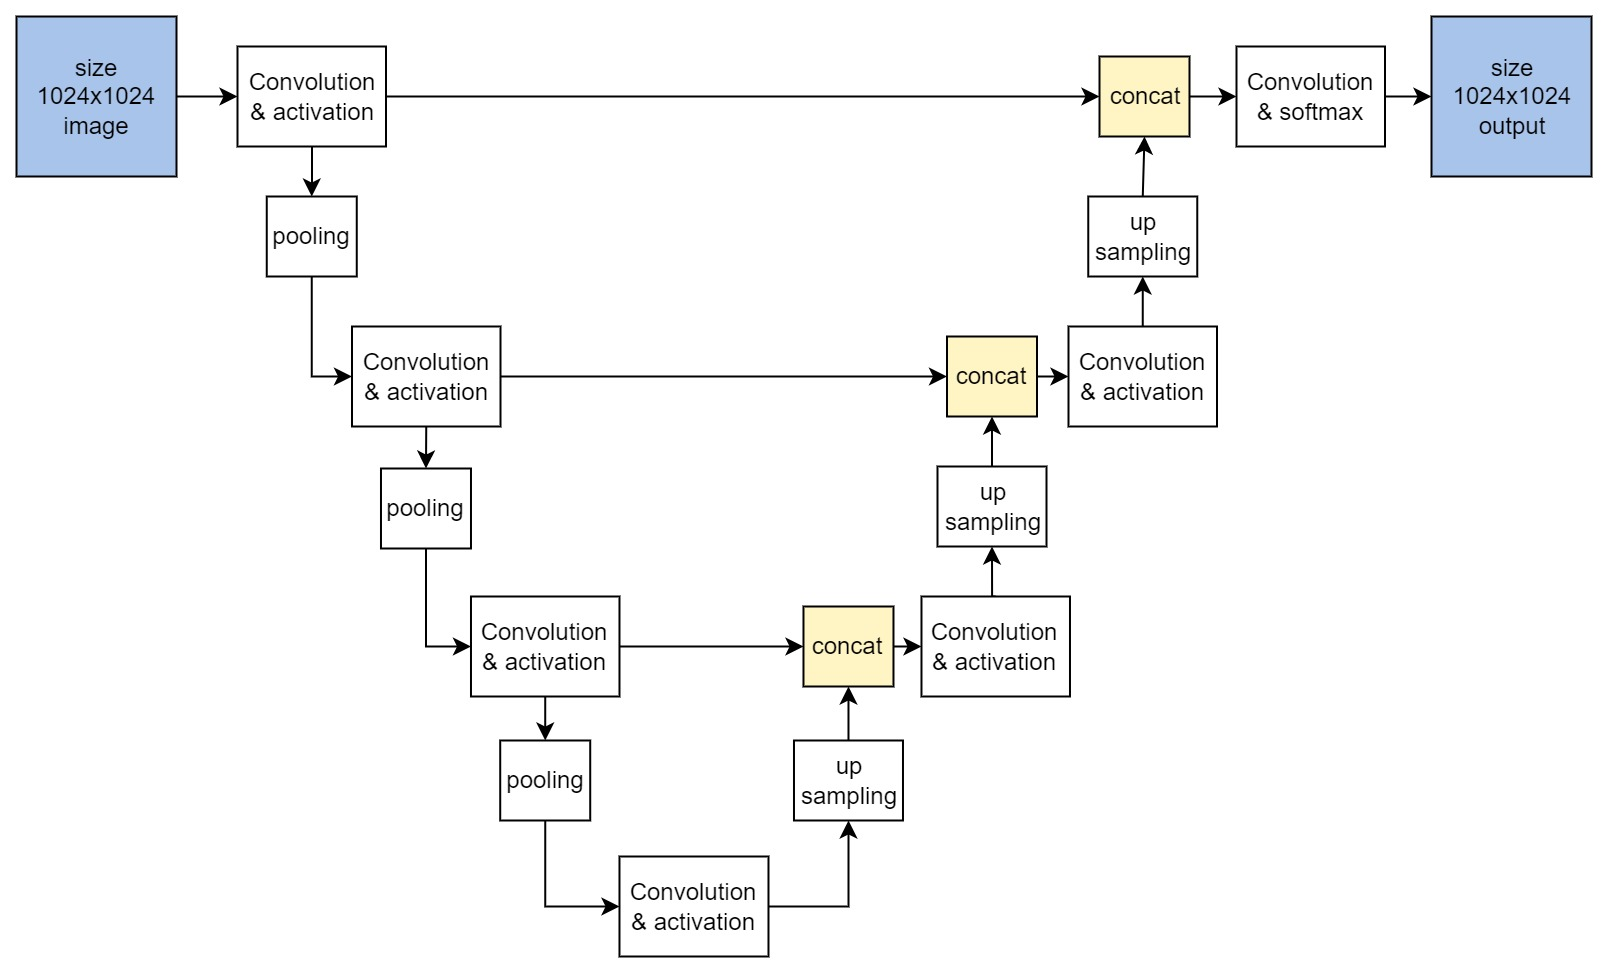
\includegraphics[height=220pt]{images/unet.jpg}
    \caption{initial UNet architecture. Redrawn from \cite{ronneberger2015u}}
    \label{fig:unet}
\end{figure}

Semantic segmentation tasks have greatly benefited from deep models because deeper CNN layers can extract more advanced semantic information\cite{Girshick_2014_CVPR}. But deep models also have a degradation problem: when we keep stacking the CNN layer, accuracy is saturated and then degrades rapidly and is not due to overfitting so only reduce the number of parameters in the CNN model cannot solve this problem. ResNet architecture greatly addressed this degradation problem by introducing residual learning and thus can stack more layers and implement deeper CNN models.\cite{he2016deep}. Figure \ref{fig:resnet} illustrates a residual learning block of ResNet. We can see that the residual learning is implemented through "shortcut connections": the output is added to the output of two convolutional layers. 

\begin{figure}[H]
    \centering
    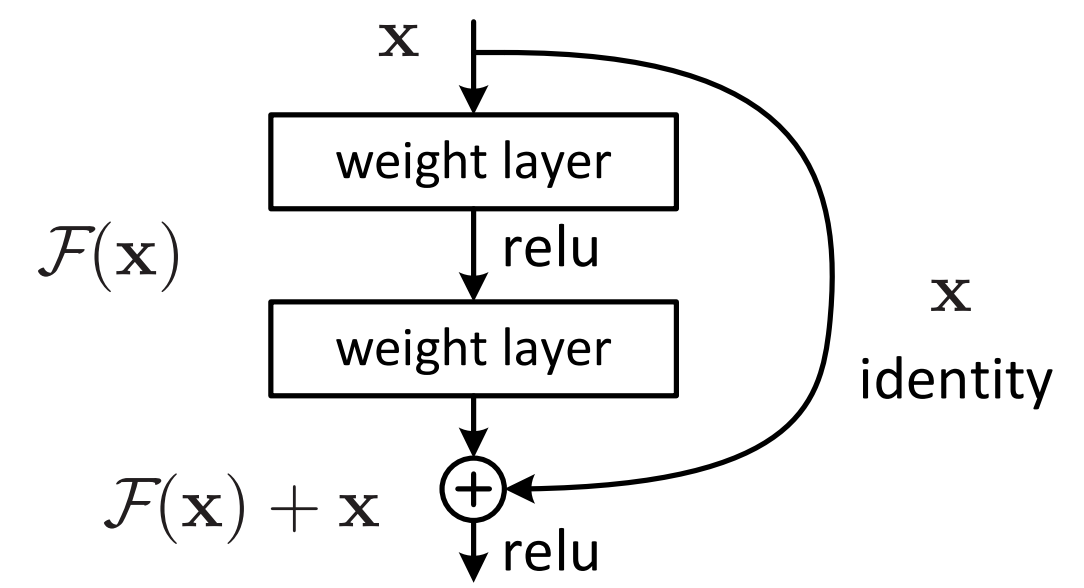
\includegraphics[height=100pt]{images/resnet.png}
    \caption{Residual learning block of ResNet.\cite{he2016deep}}
    \label{fig:resnet}
\end{figure}

For the segmentation task we chose ResNet101 (101-layer ResNet) as our CNN encoder, and the whole CNN architecture was implemented through a PyTorch\cite{NEURIPS2019_9015} based open-source tool: dhSegment\cite{oliveiraseguinkaplan2018dhsegment}.

The activation function is an indispensable part of the CNN model because it introduces nonlinear factors and gives the model ability to fit complex nonlinear problems in the real life. Sigmoid and rectified linear unit (ReLU) are two classic activation functions and have been extensively utilized in the semantic segmentation task. Using the sigmoid function may produce a gradient disappearance phenomenon, especially when we use deep CNN models, and thus result in bad prediction results. In this project, we use ReLU as our activation function. The ReLU function is shown below.

\begin{equation}
    x = max(0, x)
\end{equation}


We trained our CNN model for 60 epochs with batch size 2, and the number of accumulation step 3.  We choose Adam as our learning optimizer a set initial learning rate of $5x10^{-5}$ with an exponential decay scheduler with decay factor $\gamma=0.9999$. With the decay scheduler, after each learning step, the learning rate updates and times the decay factor $\gamma$ and thus will slowly reduce with step number growing. Figure \ref{fig:learning_rate} and equation \ref{eq:lr} shows the relationship between learning rate and number of learning steps. The whole training experienced about 50.4k and at the last learning step the learning rate reduced to $3.23x10^{-7}$.



\begin{equation}
    lr_{i+1}=lr_{i} * \gamma
    \label{eq:lr}
\end{equation}

\begin{figure}[H]
    \centering
    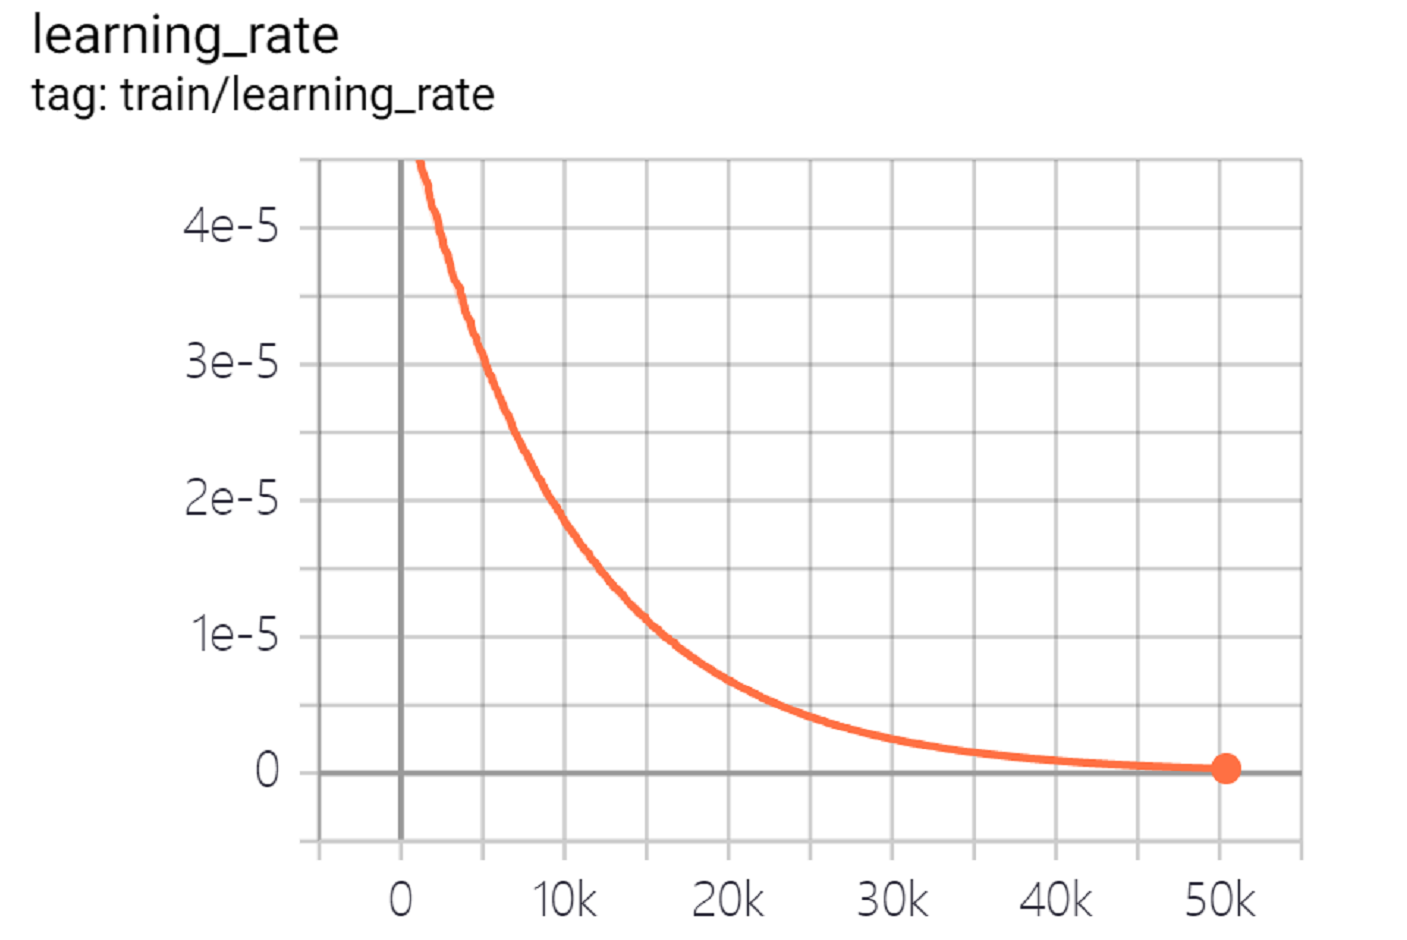
\includegraphics[height=120pt]{images/lr.png}
    \caption{Learning rate changing with training steps.}
    \label{fig:learning_rate}
\end{figure}


We use intersection over union (IoU), precision, and recall to quantify the prediction performance. After each training epoch, we use the validation set to validate our model and save the model parameter when the MIoU of the validation is higher than the current maximum MIoU.


\subsection{result}
After 60 epochs of training, we got the model with maximum MIoU at 0.9018, the IoU of the class "edge" has reached 0.8080, and precision and recall of "edge" are close to 0.9. Table \ref{tab:my_label} shows the details of the metrics value.

\begin{table}[htbp]
    \centering
    \caption{Performance achieved with the trained model.}
    \begin{tabular}{c|c|c}
    \hline
    & & \\
    Metric & Class & Value \\
    \hline
    \multirow{IoU} 
        & \textbf{Mean} & \textbf{0.9018}  \\
        & Edge & 0.8080  \\
        & Background & 0.9956  \\
    \hline
    \multirow{Precision} 
        & \textbf{Mean} & \textbf{0.9399}  \\
        & Edge & 0.8816 \\
        & Background & 0.9981 \\
    \hline
    \multirow{Recall} 
        & \textbf{Mean} & \textbf{0.9519}  \\
        & Edge & 0.9063  \\
        & Background & 0.9975 \\
    \hline
    
    \end{tabular}
    
    \label{tab:my_label}
\end{table}

Figure \ref{fig:pre_res} shows some examples of the prediction outputs in the test set. Comparing the ground truth - annotation results (Figure \ref{fig:pre_res} (b)) with the CNN model prediction outputs (Figure \ref{fig:pre_res} (c)) we can observe that the model prediction outputs are nearly identical to the corresponding ground truth, thus the model have a great performance on the test set: it predicted almost all of the road networks, buildings, wharves (Figure \ref{fig:pre_res} 2.(a-c)), rivers (Figure \ref{fig:pre_res} 5.(a-c)) and other annotated objects with high accuracy. 

But as we thought before, those texts' overlapping prediction objects indeed result in prediction errors, and the overlapped regions are not predicted accurately (Figure \ref{fig:pre_res} 4. (a-c)). Also, there are some little circles in some of the road networks, the prediction results have some gaps at the circle location (Figure \ref{fig:pre_res} 2. (a-c), 3. (a-c), 5. (a-c)).

\begin{figure}[H]
    \centering
    \rotatebox{90}{\scriptsize{~~~~~~~~~~~~~~~~~~~~~~~~1. }}
    \begin{subfigure}[b]{.28\textwidth}
		\begin{minipage}[t]{1\linewidth}
			\centering
			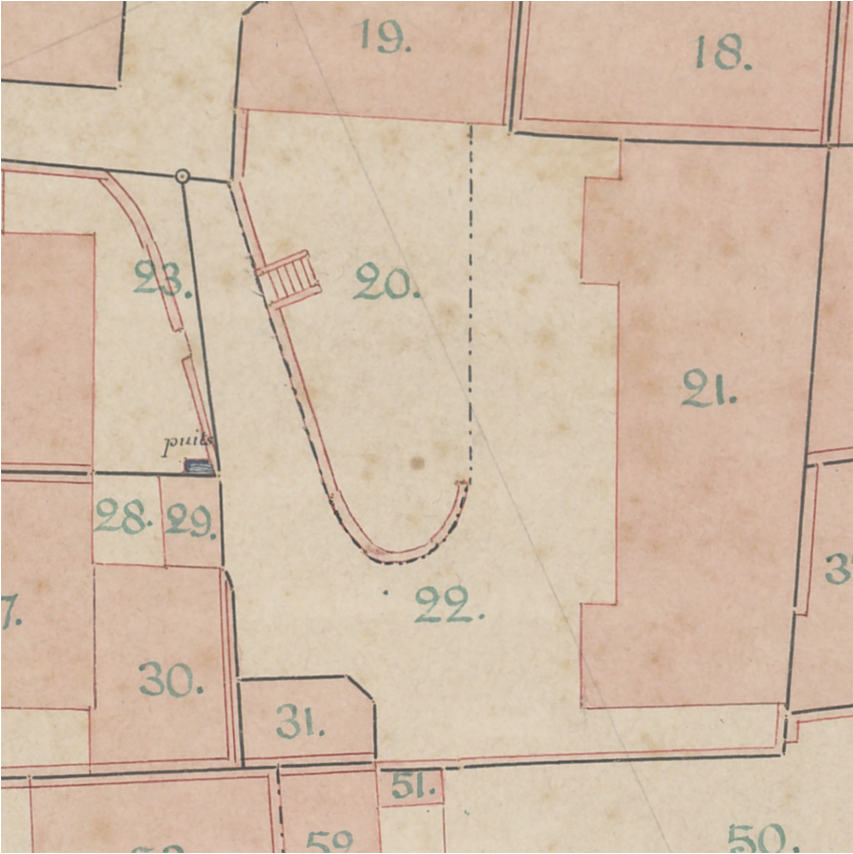
\includegraphics[width=1\linewidth]{images/patches/img3.png}
		\end{minipage}
	\end{subfigure}
	\begin{subfigure}[b]{.28\textwidth}
		\begin{minipage}[t]{1\linewidth}
			\centering
			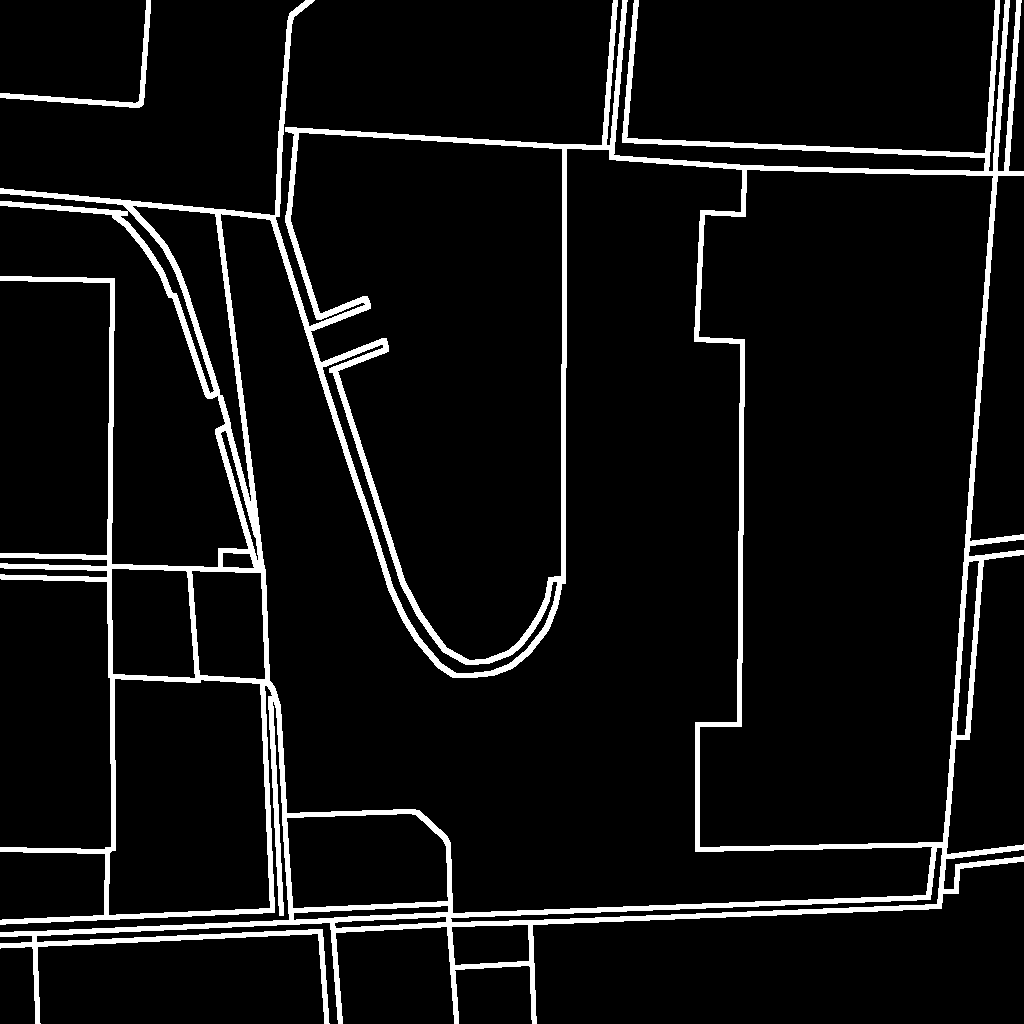
\includegraphics[width=1\linewidth]{images/patches/gt3.png}
		\end{minipage}
	\end{subfigure}
	\begin{subfigure}[b]{.28\textwidth}
		\begin{minipage}[t]{1\linewidth}
			\centering
			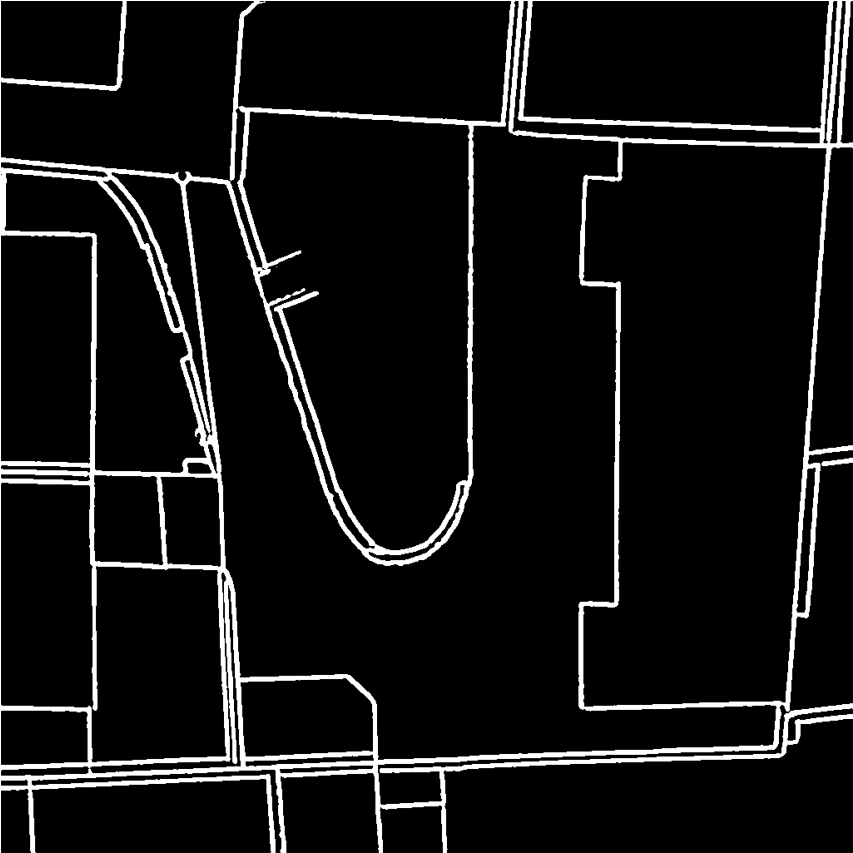
\includegraphics[width=1\linewidth]{images/patches/pre3.png}
		\end{minipage}
	\end{subfigure}


 	\vspace{+2mm}
    \setcounter{subfigure}{0}
	
	\rotatebox{90}{\scriptsize{~~~~~~~~~~~~~~~~~~~~~~~~2. }}
    \begin{subfigure}[b]{.28\textwidth}
		\begin{minipage}[t]{1\linewidth}
			\centering
			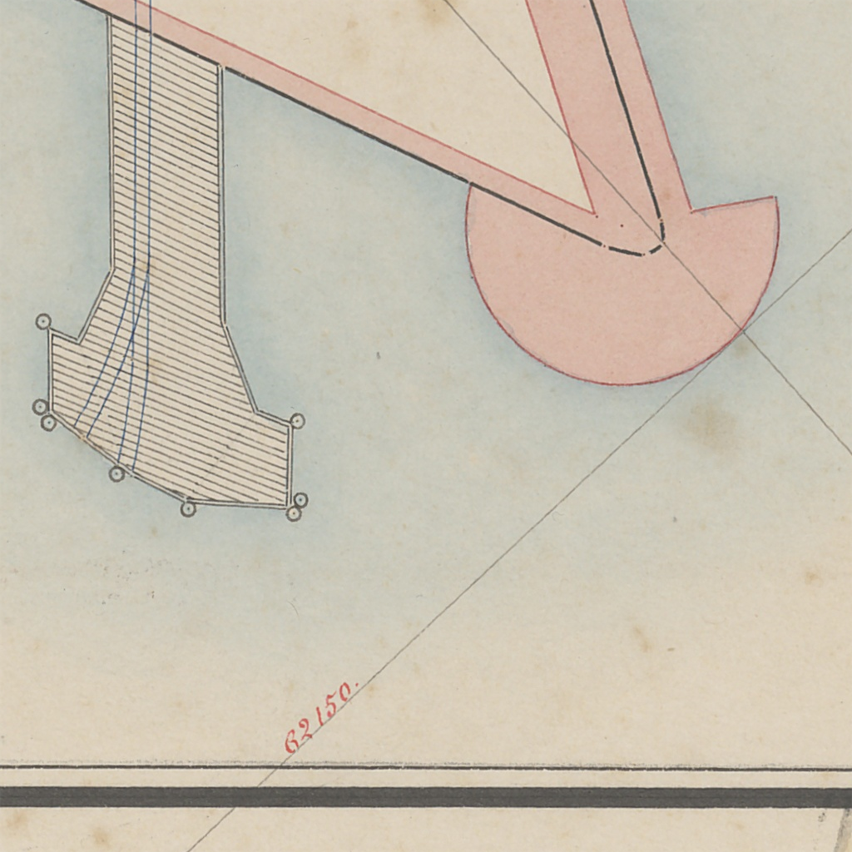
\includegraphics[width=1\linewidth]{images/patches/img8.png}
		\end{minipage}
	\end{subfigure}
	\begin{subfigure}[b]{.28\textwidth}
		\begin{minipage}[t]{1\linewidth}
			\centering
			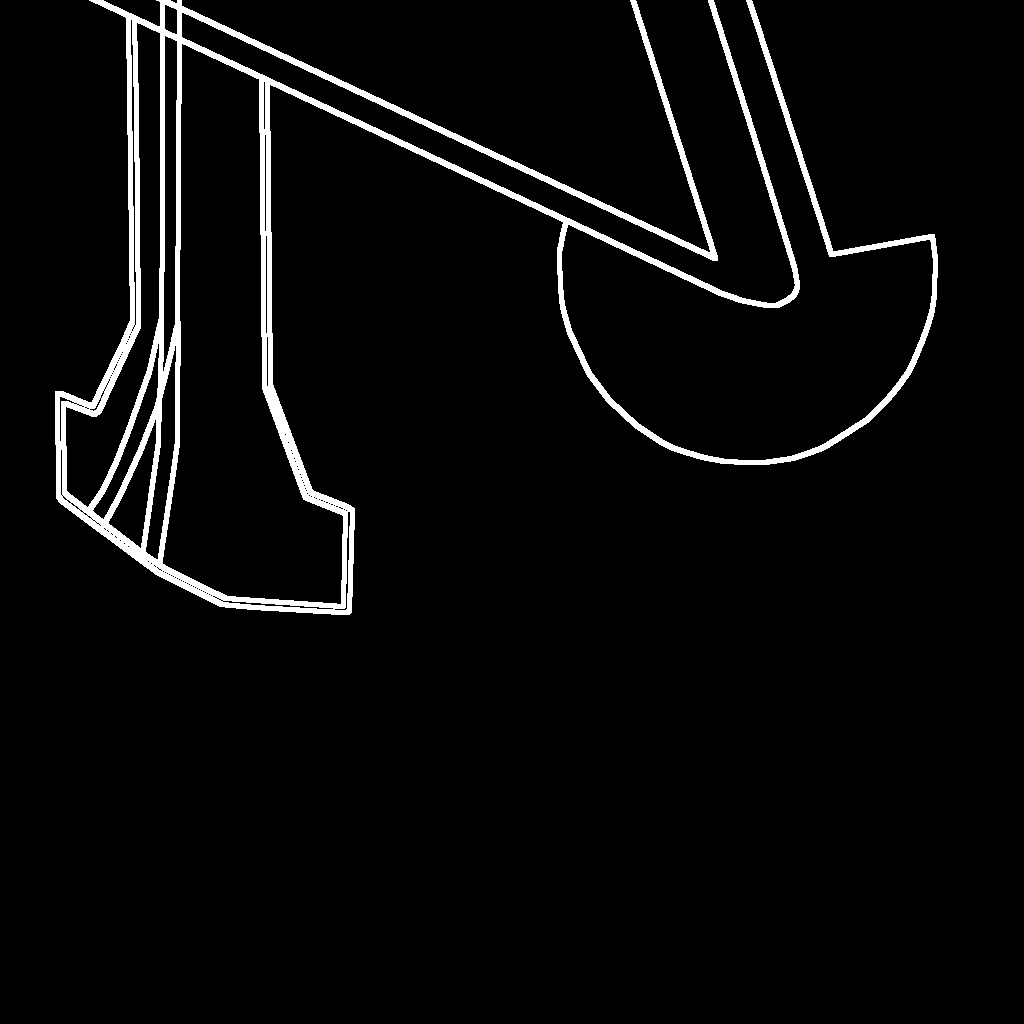
\includegraphics[width=1\linewidth]{images/patches/gt8.png}
		\end{minipage}
	\end{subfigure}
	\begin{subfigure}[b]{.28\textwidth}
		\begin{minipage}[t]{1\linewidth}
			\centering
			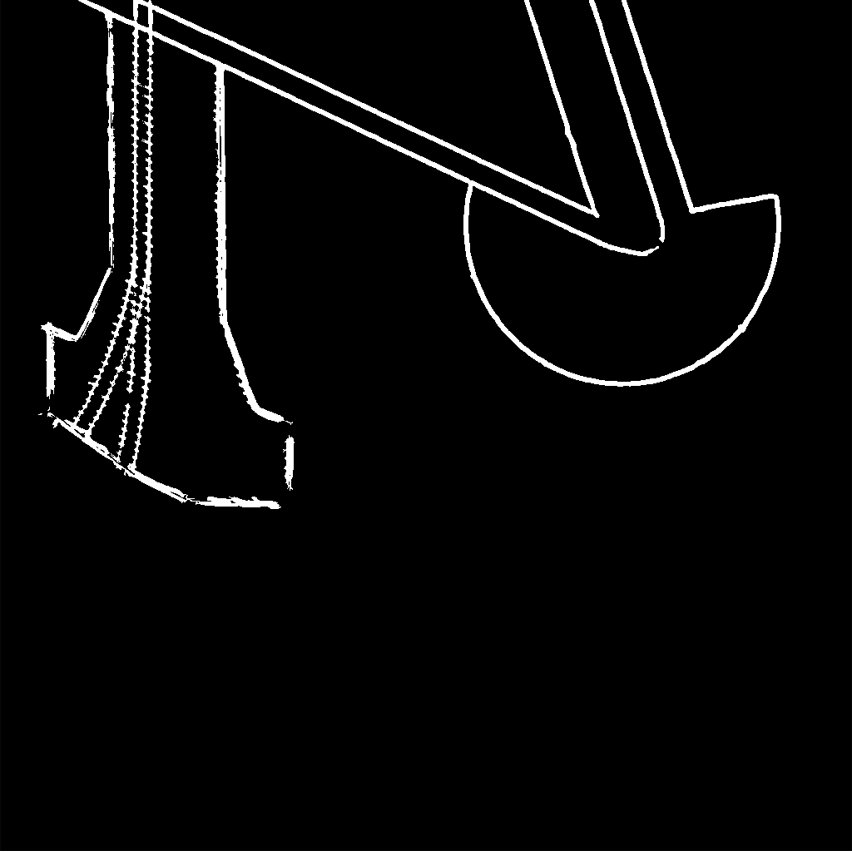
\includegraphics[width=1\linewidth]{images/patches/pre8.png}
		\end{minipage}
	\end{subfigure}

	\vspace{+2mm}
    \setcounter{subfigure}{0}
    
        \rotatebox{90}{\scriptsize{~~~~~~~~~~~~~~~~~~~~~~~~3. }}
    \begin{subfigure}[b]{.28\textwidth}
		\begin{minipage}[t]{1\linewidth}
			\centering
			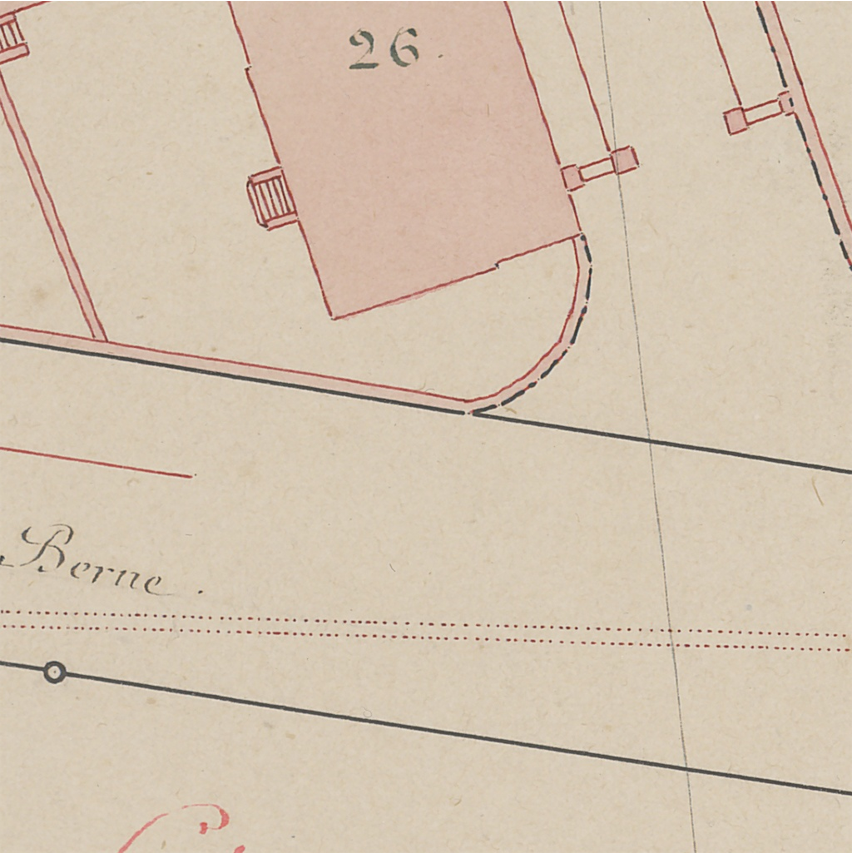
\includegraphics[width=1\linewidth]{images/patches/img6.png}
		\end{minipage}
	\end{subfigure}
	\begin{subfigure}[b]{.28\textwidth}
		\begin{minipage}[t]{1\linewidth}
			\centering
			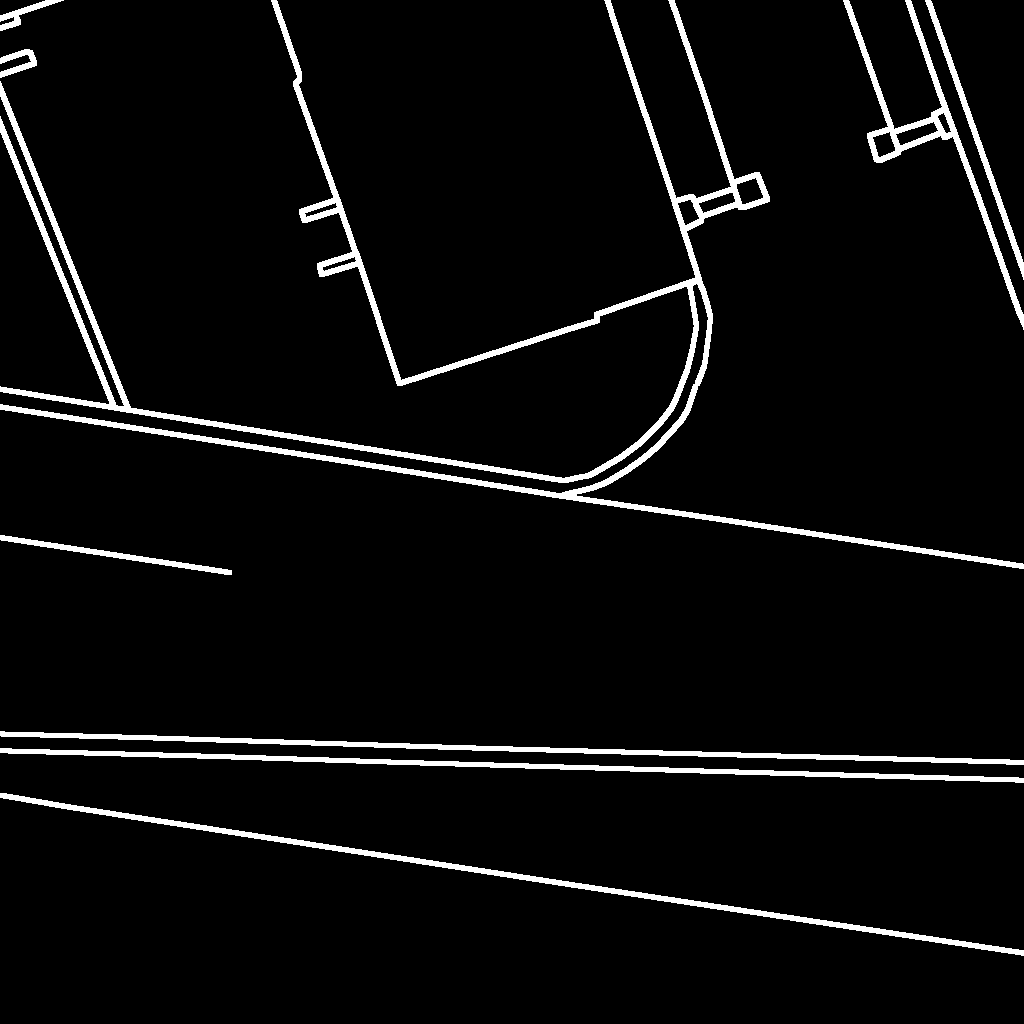
\includegraphics[width=1\linewidth]{images/patches/gt6.png}
		\end{minipage}
	\end{subfigure}
	\begin{subfigure}[b]{.28\textwidth}
		\begin{minipage}[t]{1\linewidth}
			\centering
			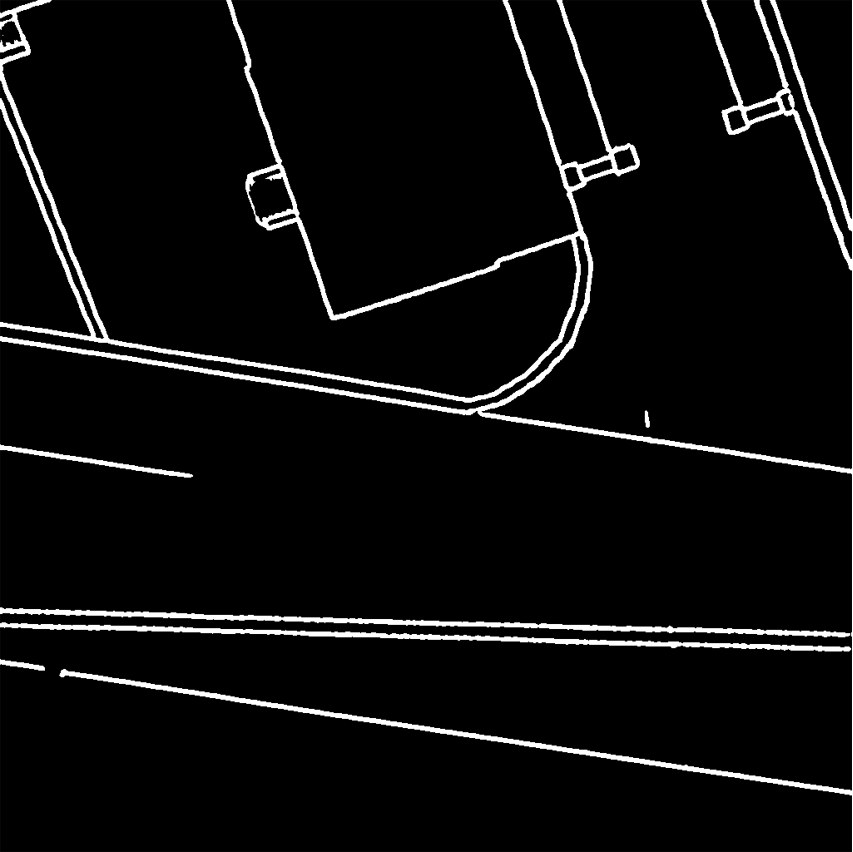
\includegraphics[width=1\linewidth]{images/patches/pre6.png}
		\end{minipage}
	\end{subfigure}

	\vspace{+2mm}
    \setcounter{subfigure}{0}
    
    \rotatebox{90}{\scriptsize{~~~~~~~~~~~~~~~~~~~~~~~~4. }}
    \begin{subfigure}[b]{.28\textwidth}
		\begin{minipage}[t]{1\linewidth}
			\centering
			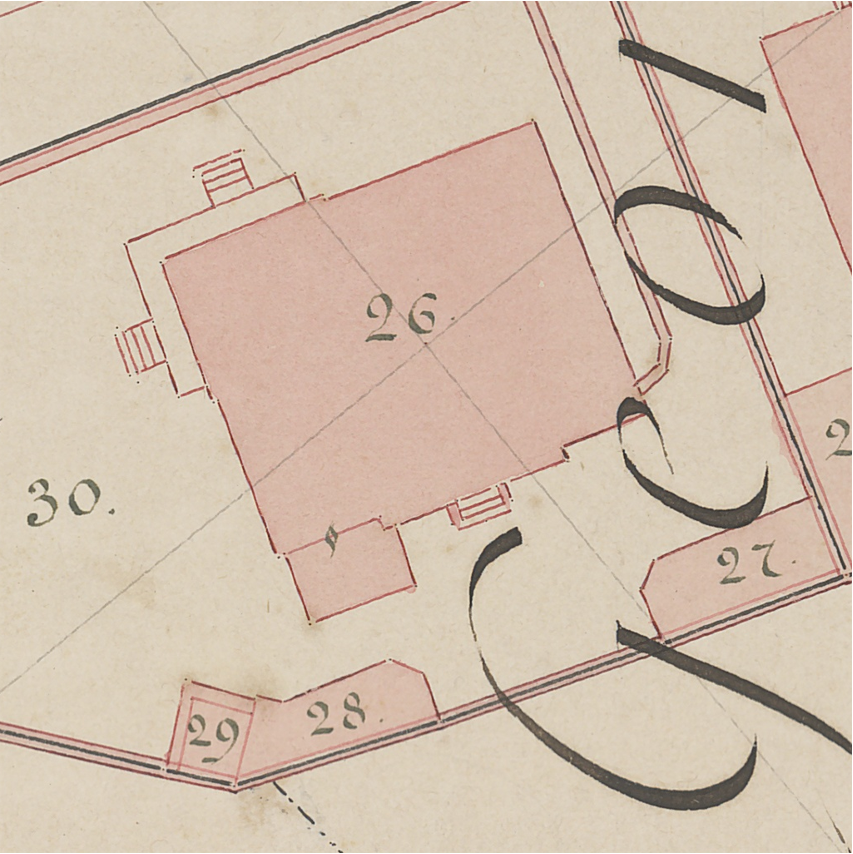
\includegraphics[width=1\linewidth]{images/patches/img7.png}
		\end{minipage}
	\end{subfigure}
	\begin{subfigure}[b]{.28\textwidth}
		\begin{minipage}[t]{1\linewidth}
			\centering
			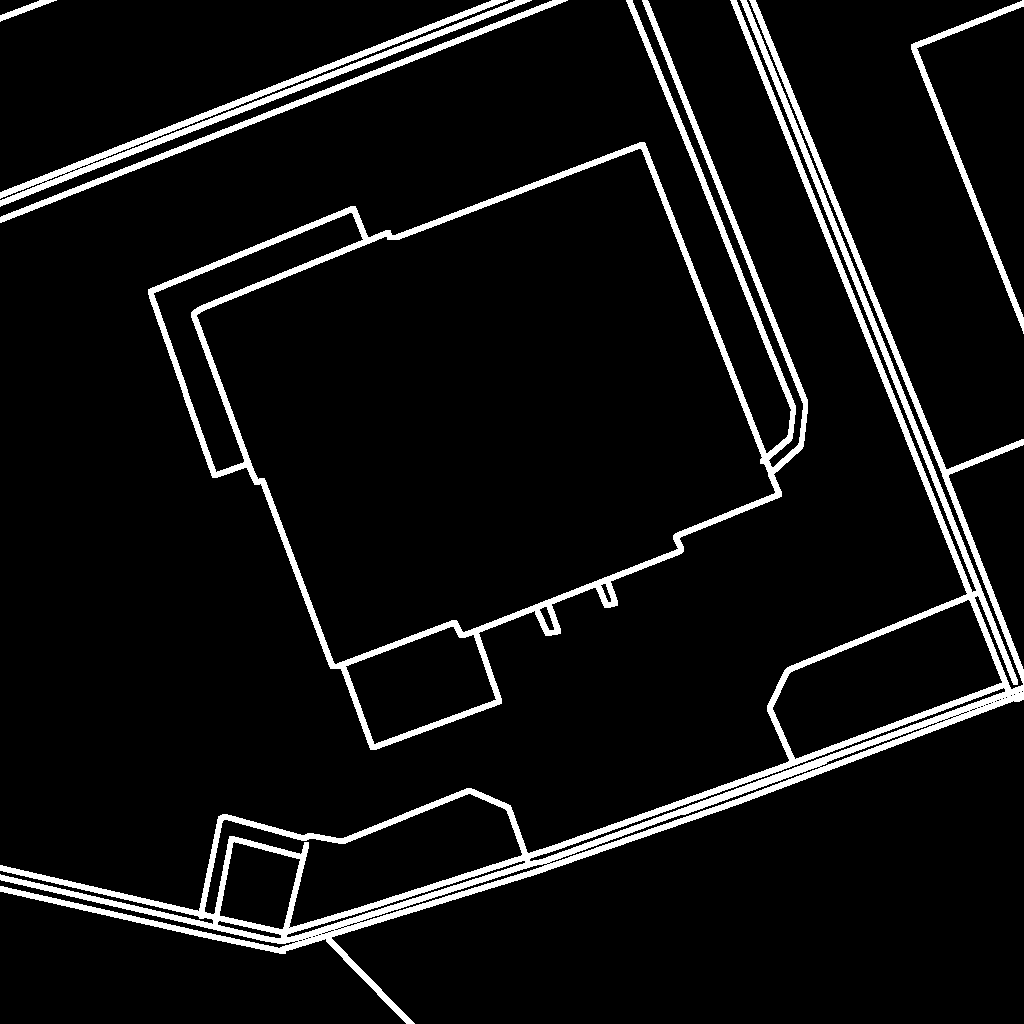
\includegraphics[width=1\linewidth]{images/patches/gt7.png}
		\end{minipage}
	\end{subfigure}
	\begin{subfigure}[b]{.28\textwidth}
		\begin{minipage}[t]{1\linewidth}
			\centering
			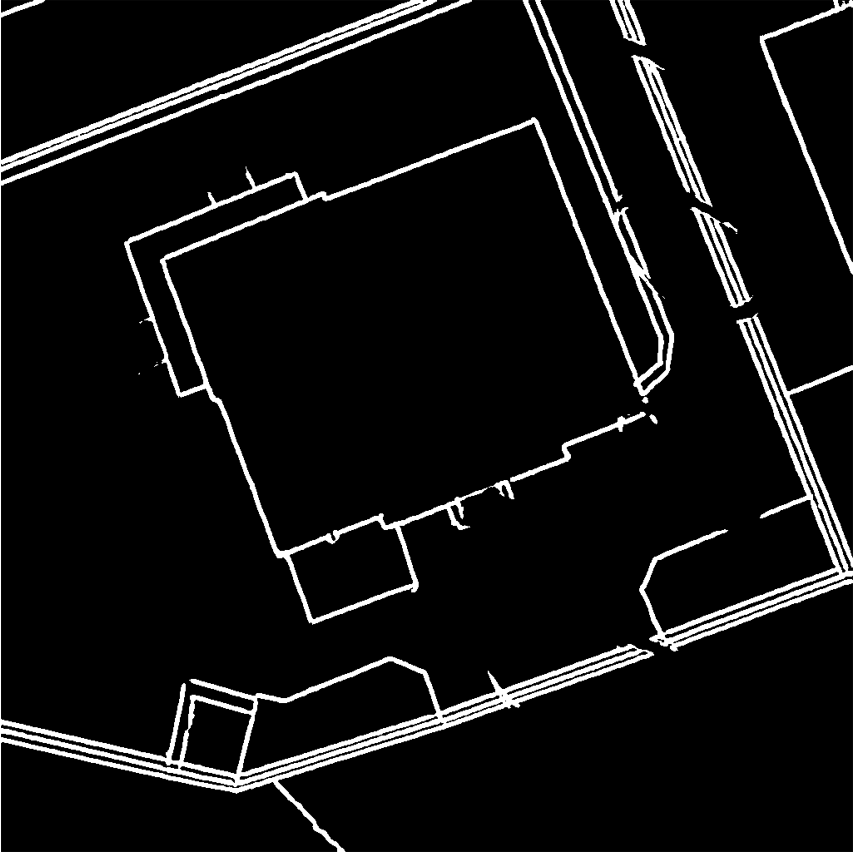
\includegraphics[width=1\linewidth]{images/patches/pre7.png}
		\end{minipage}
	\end{subfigure}

	\vspace{+2mm}
    \setcounter{subfigure}{0}
	
	
	
	
 
    % 第二行图片展示
    \rotatebox{90}{\scriptsize{~~~~~~~~~~~~~~~~~~~~~~~~5. }}
    \begin{subfigure}[b]{.28\textwidth}
        % 左标题2
		
		\begin{minipage}[t]{1\linewidth}
			\centering
			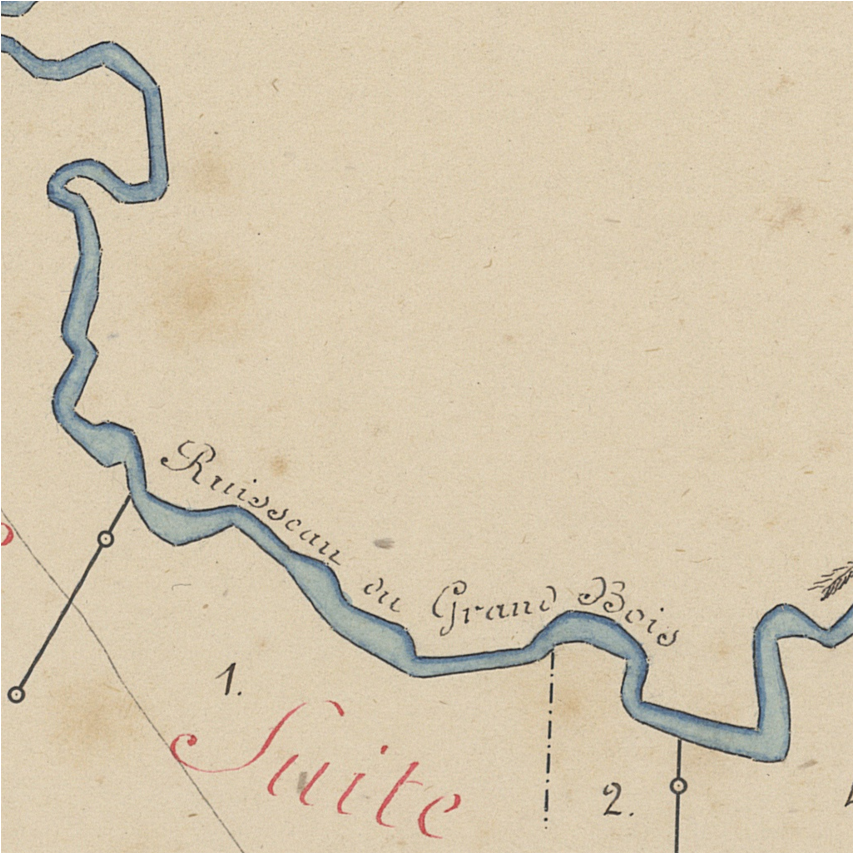
\includegraphics[width=1\linewidth]{images/patches/img10.png}
			\caption{Image}
		\end{minipage}
	\end{subfigure}
	\begin{subfigure}[b]{.28\textwidth}
		\begin{minipage}[t]{1\linewidth}
			\centering
			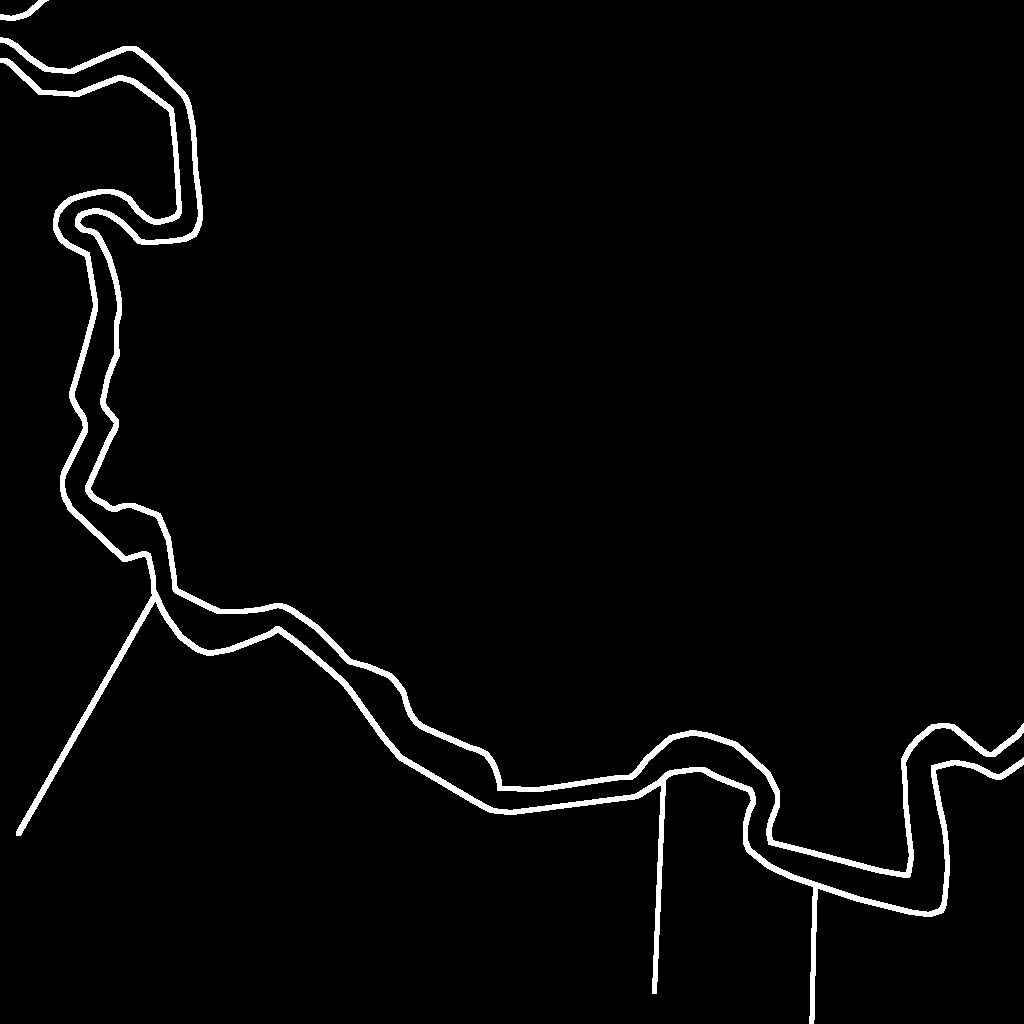
\includegraphics[width=1\linewidth]{images/patches/gt10.png}
			\caption{Ground Truth}
		\end{minipage}
	\end{subfigure}
	\begin{subfigure}[b]{.28\textwidth}
		\begin{minipage}[t]{1\linewidth}
			\centering
			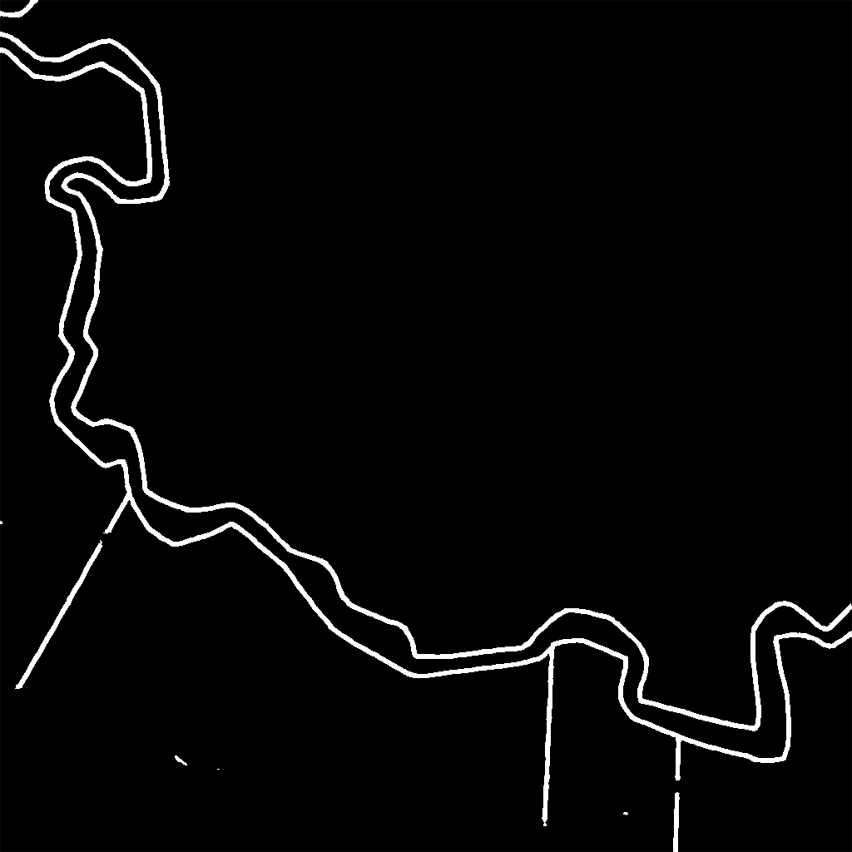
\includegraphics[width=1\linewidth]{images/patches/pre10.png}
		    \caption{Prediction output}
		\end{minipage}
	\end{subfigure}
	
    \caption{Patches of prediction results}
    \label{fig:pre_res}
\end{figure}



\subsection{Prediction map reconstitution}
Now we have a good performance model to predict “edges” from 1024x1024-size patches. Now we want to reconstitute the prediction result of the whole map for polygon recovery in the next chapter.

We patched these 12 annotated maps to size 1024x1024 with an overlap of 200 and put them into the trained model to get patches of prediction results, then we reconstitute those predicted patches to the whole prediction map. For the overlapping domain, we averaged the prediction probabilities and got the final probability. Figure \ref{fig:original-reconstitution} shows an example of the reconstitution result. We can see that the CNN model well predicted the original map.

\begin{figure}[H]
    \centering
	\begin{subfigure}[b]{.32\textwidth}
		% include first image
		\centering
		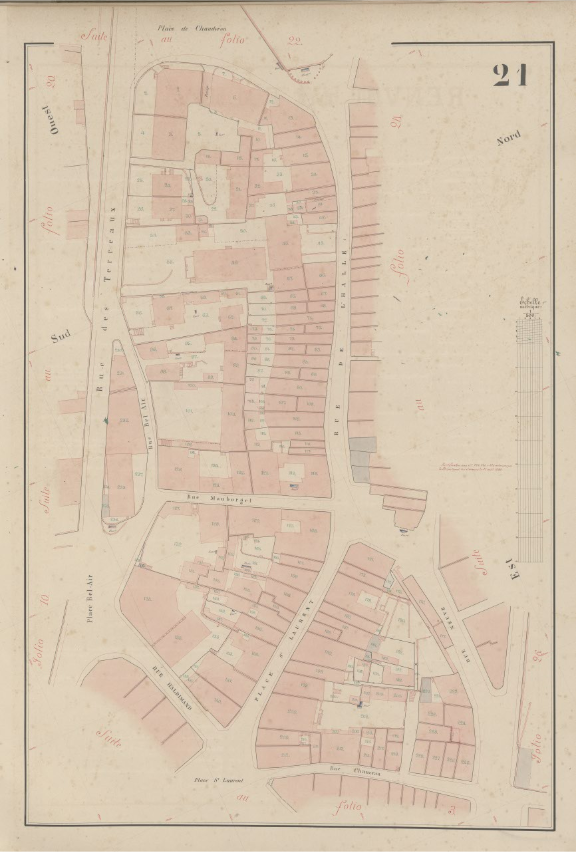
\includegraphics[width=1\linewidth]{images/original_image.png}  
		\label{fig:original-img}
	\end{subfigure}
	\begin{subfigure}[b]{.32\textwidth}
		% include second image
		\centering
		\includegraphics[width=1\linewidth]{images/original_gt.png}  
		\label{fig:original-gt}
	\end{subfigure}
	\begin{subfigure}[b]{.32\textwidth}
		% include second image
		\centering
		\includegraphics[width=1\linewidth]{images/original_prediction.png}  
		\label{fig:original-pre}
	\end{subfigure}
	
	\begin{subfigure}[b]{.32\textwidth}
		% include first image
		\centering
		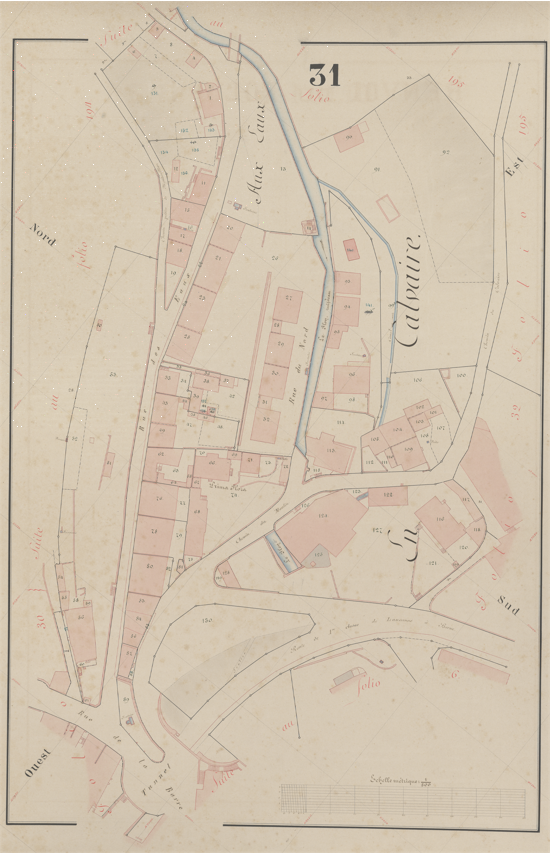
\includegraphics[width=1\linewidth]{images/original_image2.png}  
		\label{fig:original-img}
		\caption{Original image}
	\end{subfigure}
	\begin{subfigure}[b]{.32\textwidth}
		% include second image
		\centering
		\includegraphics[width=1\linewidth]{images/original_gt2.png}  
		\label{fig:original-gt}
		\caption{Ground truth}
	\end{subfigure}
	\begin{subfigure}[b]{.32\textwidth}
		% include second image
		\centering
		\includegraphics[width=1\linewidth]{images/original_prediction2.png}  
		\label{fig:original-pre}
		\caption{Prediction outputs}
	\end{subfigure}
	
	\caption{Prediction reconstitution examples of annotated map.}
	\label{fig:original-reconstitution}
\end{figure}


To test the robustness of our trained model, We also predicted and reconstituted additional 12 unannotated maps and all of the results have shown great prediction performance. Two examples of the prediction outputs are shown in Figure \ref{fig:additional-reconstitution}. The results indicate that the CNN model has good robustness and has good performance on maps that did not exist at the training step and validation step before, so we can believe that the CNN model we trained can well predict the whole cadastre consisting of 300 historical maps of Lausanne. Next, we will use those reconstitution map predictions to begin the polygon recovery process.

\begin{figure}[H]
    \centering
	\begin{subfigure}[b]{.4\textwidth}
		% include first image
		\centering
		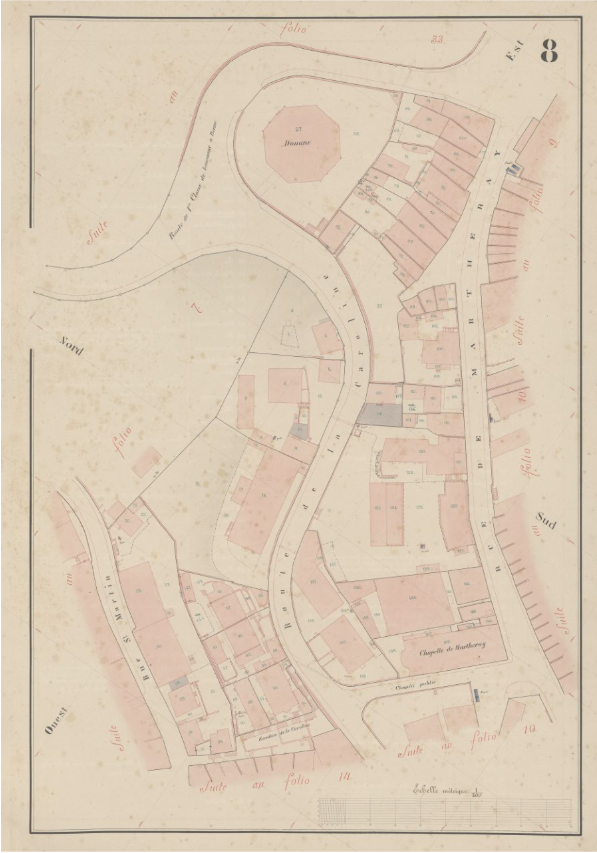
\includegraphics[width=1\linewidth]{images/additional_image.png}  
		\label{fig:original-img}
% 		\caption{Original image}
	\end{subfigure}
	\begin{subfigure}[b]{.4\textwidth}
		% include second image
		\centering
		\includegraphics[width=1\linewidth]{images/additional_prediction.png}  
		\label{fig:original-pre}
% 		\caption{Prediction outputs}
	\end{subfigure}
	

	\begin{subfigure}[b]{.4\textwidth}
		% include first image
		\centering
		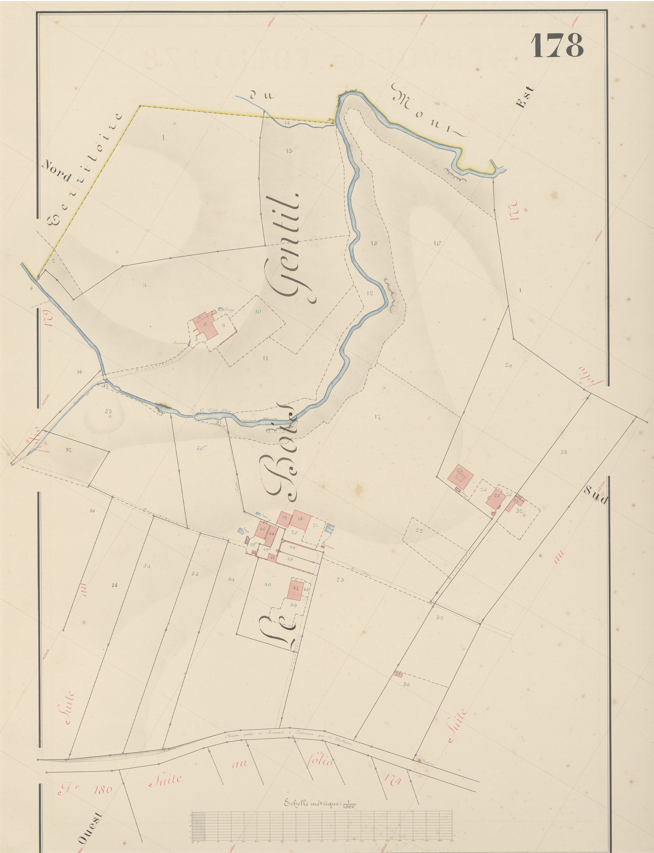
\includegraphics[width=1\linewidth]{images/additional_image2.png}  
		\label{fig:original-img}
		\caption{Original image}
	\end{subfigure}
	\begin{subfigure}[b]{.4\textwidth}
		% include second image
		\centering
		\includegraphics[width=1\linewidth]{images/additional_prediction2.png}  
		\label{fig:original-pre}
		\caption{Prediction outputs}
	\end{subfigure}
	
	
	\caption{Prediction reconstitution examples of map without annotation and training.}
	\label{fig:additional-reconstitution}
\end{figure}


\section{Polygon Recovery}
In the semantic segmentation chapter, we trained the CNN model to predict edges from map patches and reconstituted the prediction results of each map. In this chapter, we will find an automatic computer vision method to recover polygons from these reconstitution prediction outputs. With the polygon-recovered results, people can just manual-label the polygons to generate vector images, like the "shapefile (.shp)" format, in the future.

Polygon recovery is to judge whether a region should be split into little regions and determine the boundaries of the region if we decide to split, and those determined boundaries are the boundaries of each recovered polygon. The main difficulty of polygon recovery is that not all of the "edges" in the reconstituted prediction maps are closed: There may be some gaps in a polygon boundary due to: 1) The polygon is at the edge of the cadastre map. 2) The lines themselves in the map are not intersected in the map and the polygons are not closed in these original maps. 3) There are some gaps in a line of prediction result because of prediction error, and maybe the prediction is influenced by text descriptions in the map which overlap the prediction objects. (Figure \ref{fig:pre_res}). 

To finish the polygon recovery task, we tried two computer vision methods: watershed transformation and the Felzenswalb algorithm, both of them are provided in the Python library in scikit-image\cite{van2014scikit} "skimage.segmentation". The result of both algorithms are shown in Figure \ref{fig:watershed1}, \ref{fig:watershed2}.

\subsection{Watershed transformation}

Watershed transformation algorithm is a morphological-based tool for image segmentation which is originally proposed by Digabel and Lantuejoul (1977) and later improved by Li et. al. (2003)\cite{khiyal2009modified, li2003improved}. The idea of watershed transformation is that it thinks of an image as a topographic map. Firstly we should choose some "catchment basins" on the map,  As water is poured at those "catchment basins", we should build dams where water from different catchment basins can meet to avoid catchment basins connecting and merging. Finally, those lines of the watershed are defined by catchment areas divided by those dams at the highest level where water can meet together and the watershed lines are regarded as boundaries of segmented regions, and thus the polygon recovering is finished.

The key point of the watershed transformation is how to choose these "catchment basins", which are usually the local lowest points (local minimum points of gray value) of the map. We can change the distance of determining local minimum points to change the number of the "catchment basins". If the determining distance is too small, there will be too many basins so that too many polygons are segmented, and a lot of polygons are necessary. On the contrary, if the determining distance is too large, the number of basins is not large enough and thus polygons cannot be well segmented. For different kinds of maps, different distances should be set for the best watershed performance.  

Figure \ref{fig:watershed1}, \ref{fig:watershed2} shows the result of the watershed transformation using different minimum basin distances of two different kinds of maps. Comparing the results of the two maps, we can observe that they have different best minimum basin distances (min\_distance=30 for Figure \ref{fig:watershed1}, min\_distance=10 for Figure \ref{fig:watershed2}). When the distance is set too small, there will be too many catchment basins so that too many polygons are segmented, and some big regions will contain many small regions with dense parallel boundaries, horizontal or vertical (Figure \ref{fig:watershed1} (c), \ref{fig:watershed2} (c)). However, when the minimum distance is too large, polygons are not segmented adequately and there exists a lot of connected regions which should be split (\ref{fig:watershed1} (e), buildings at the center of the map in Figure \ref{fig:watershed1} (e)). The results of the watershed transformation are acceptable and reasonable when the minimum distance of the catchment basin is appropriate.


\subsection{Felzenswalb algorithm}

Felzenswalb algorithm is a graph-based segmentation algorithm based on greedy clustering algorithm, which was proposed by Felzenszwalb and Huttenlocher in 2004\cite{felzenszwalb2004efficient}. At the beginning, each pixel is a vertex, and then these vertexes are gradually merged into a region, specifically an minimum spanning tree (MST) connecting the pixels in the region\cite{boykov2006graph}. At the end, the result of the segmentation is a forest consisting of some MSTs, and each MST represents a segmented region (polygon).

The key parameter of using Felzenswalb is the scale of the observation $k$, and a larger $k$ causes a preference for segmenting larger and more coarse regions, and split result is finer and regions are smaller with smaller $k$.  

Figure \ref{fig:watershed1} shows the result of Felzenswalb. We can observe that the main problem of Felzenswalb segmentation is that it often over-segment those thin long polygons like road networks, especially when the scale of observation is smaller (Figure \ref{fig:watershed1} (f), \ref{fig:watershed2} (f)), but in this case wider polygons have not encountered over-segment problem like watershed (Figure \ref{fig:watershed1} (c), \ref{fig:watershed2} (c)). When scale of observation is too larger, similar as the watershed, polygons are not segmented adequately and some regions are connected with this algorithm but in the original map they are indeed two different regions (Figure \ref{fig:watershed2} (h), \ref{fig:watershed2} (h)). The results of watershed transformation are also acceptable when we set appropriate scale of observation.


\begin{figure}[H]
    \centering
	\begin{subfigure}[b]{.3\textwidth}
		% include first image
		\centering
		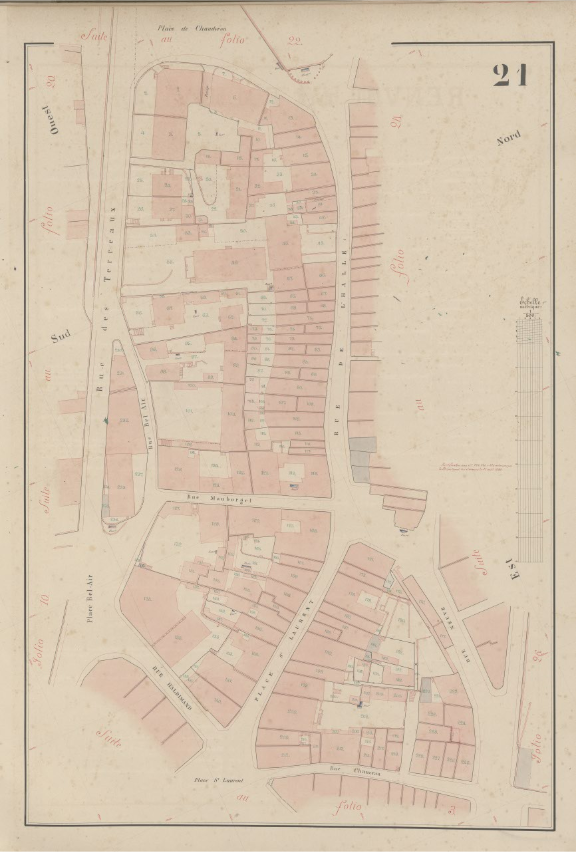
\includegraphics[width=1\linewidth]{images/original_image.png}  
		\caption{Original image}
	\end{subfigure}
	\begin{subfigure}[b]{.3\textwidth}
		% include second image
		\centering
		\includegraphics[width=1\linewidth]{images/original_gt.png}  
		\caption{CNN Prediction outputs}
	\end{subfigure}
	
    \rotatebox{90}{\small{~~~~~~~~~~~~~~~~~~~~~~~~~~~~~~1. Watershed outputs}}
	\begin{subfigure}[b]{.3\textwidth}
		% include first image
		\centering
		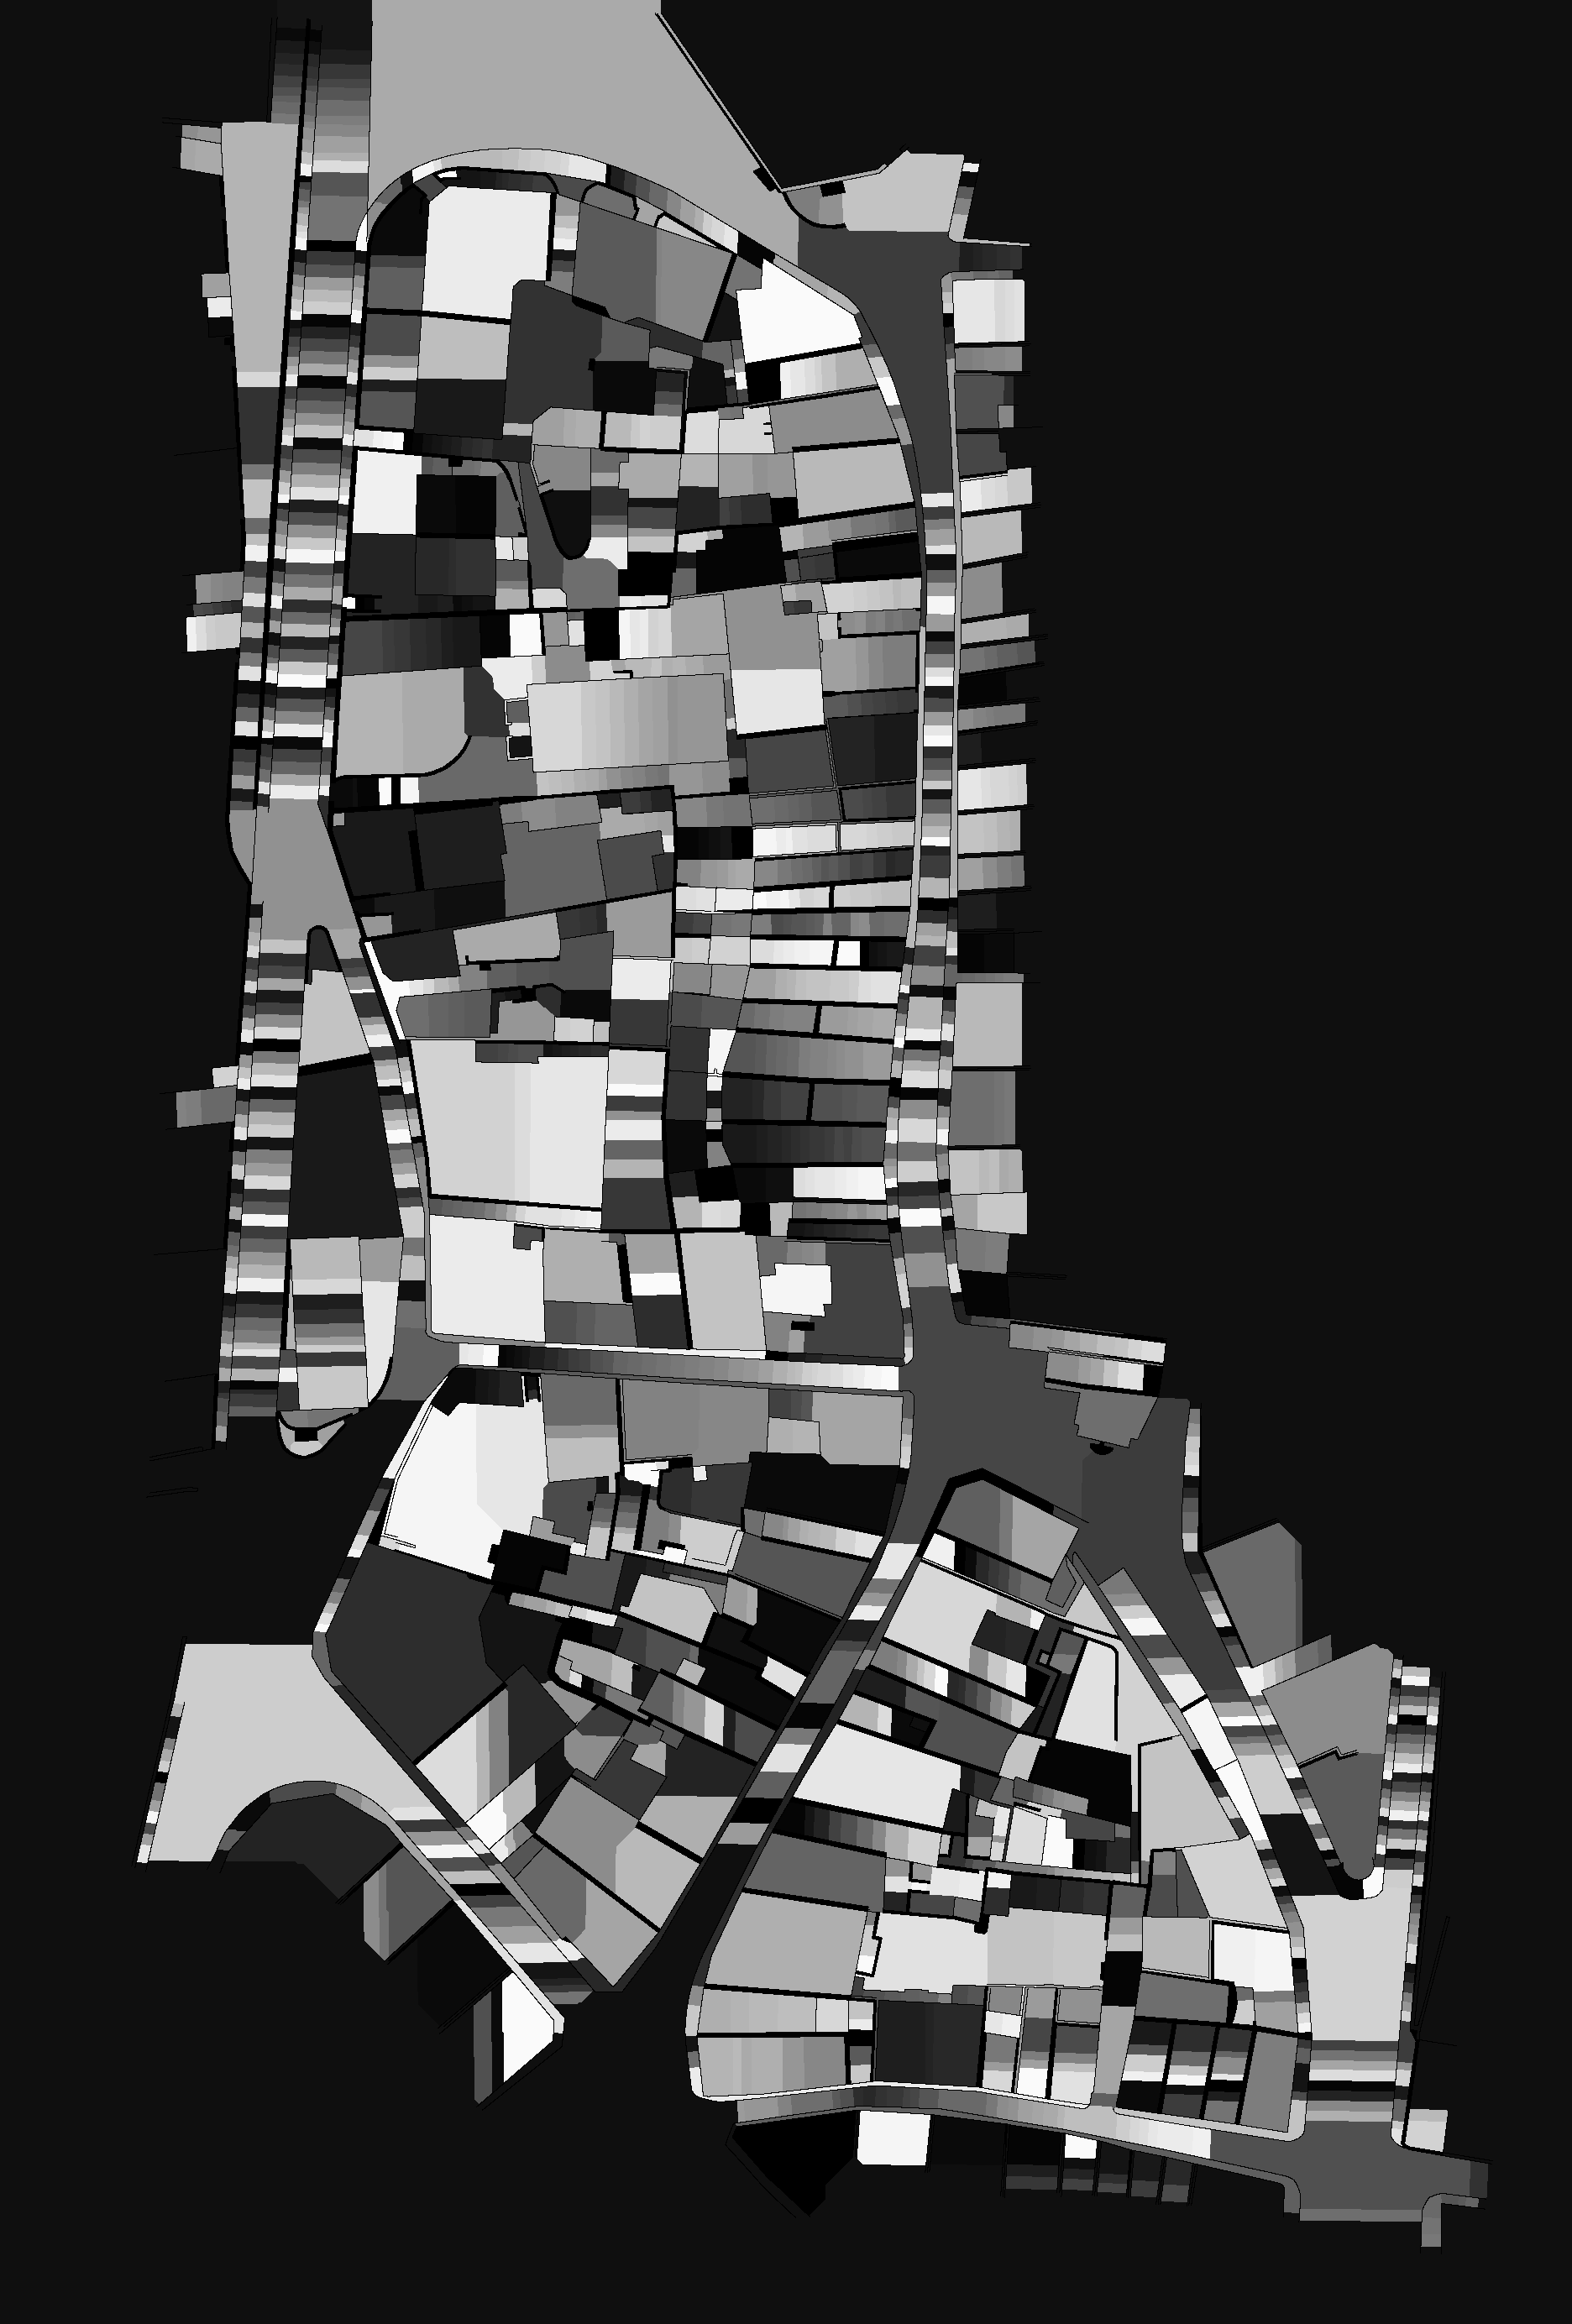
\includegraphics[width=1\linewidth]{images/polygon_recovery/watershed1_distance10_b1911.png}  
		\caption{min\_distance=10, \\ 1911 polygons}
	\end{subfigure}
	\begin{subfigure}[b]{.3\textwidth}
		% include second image
		\centering
		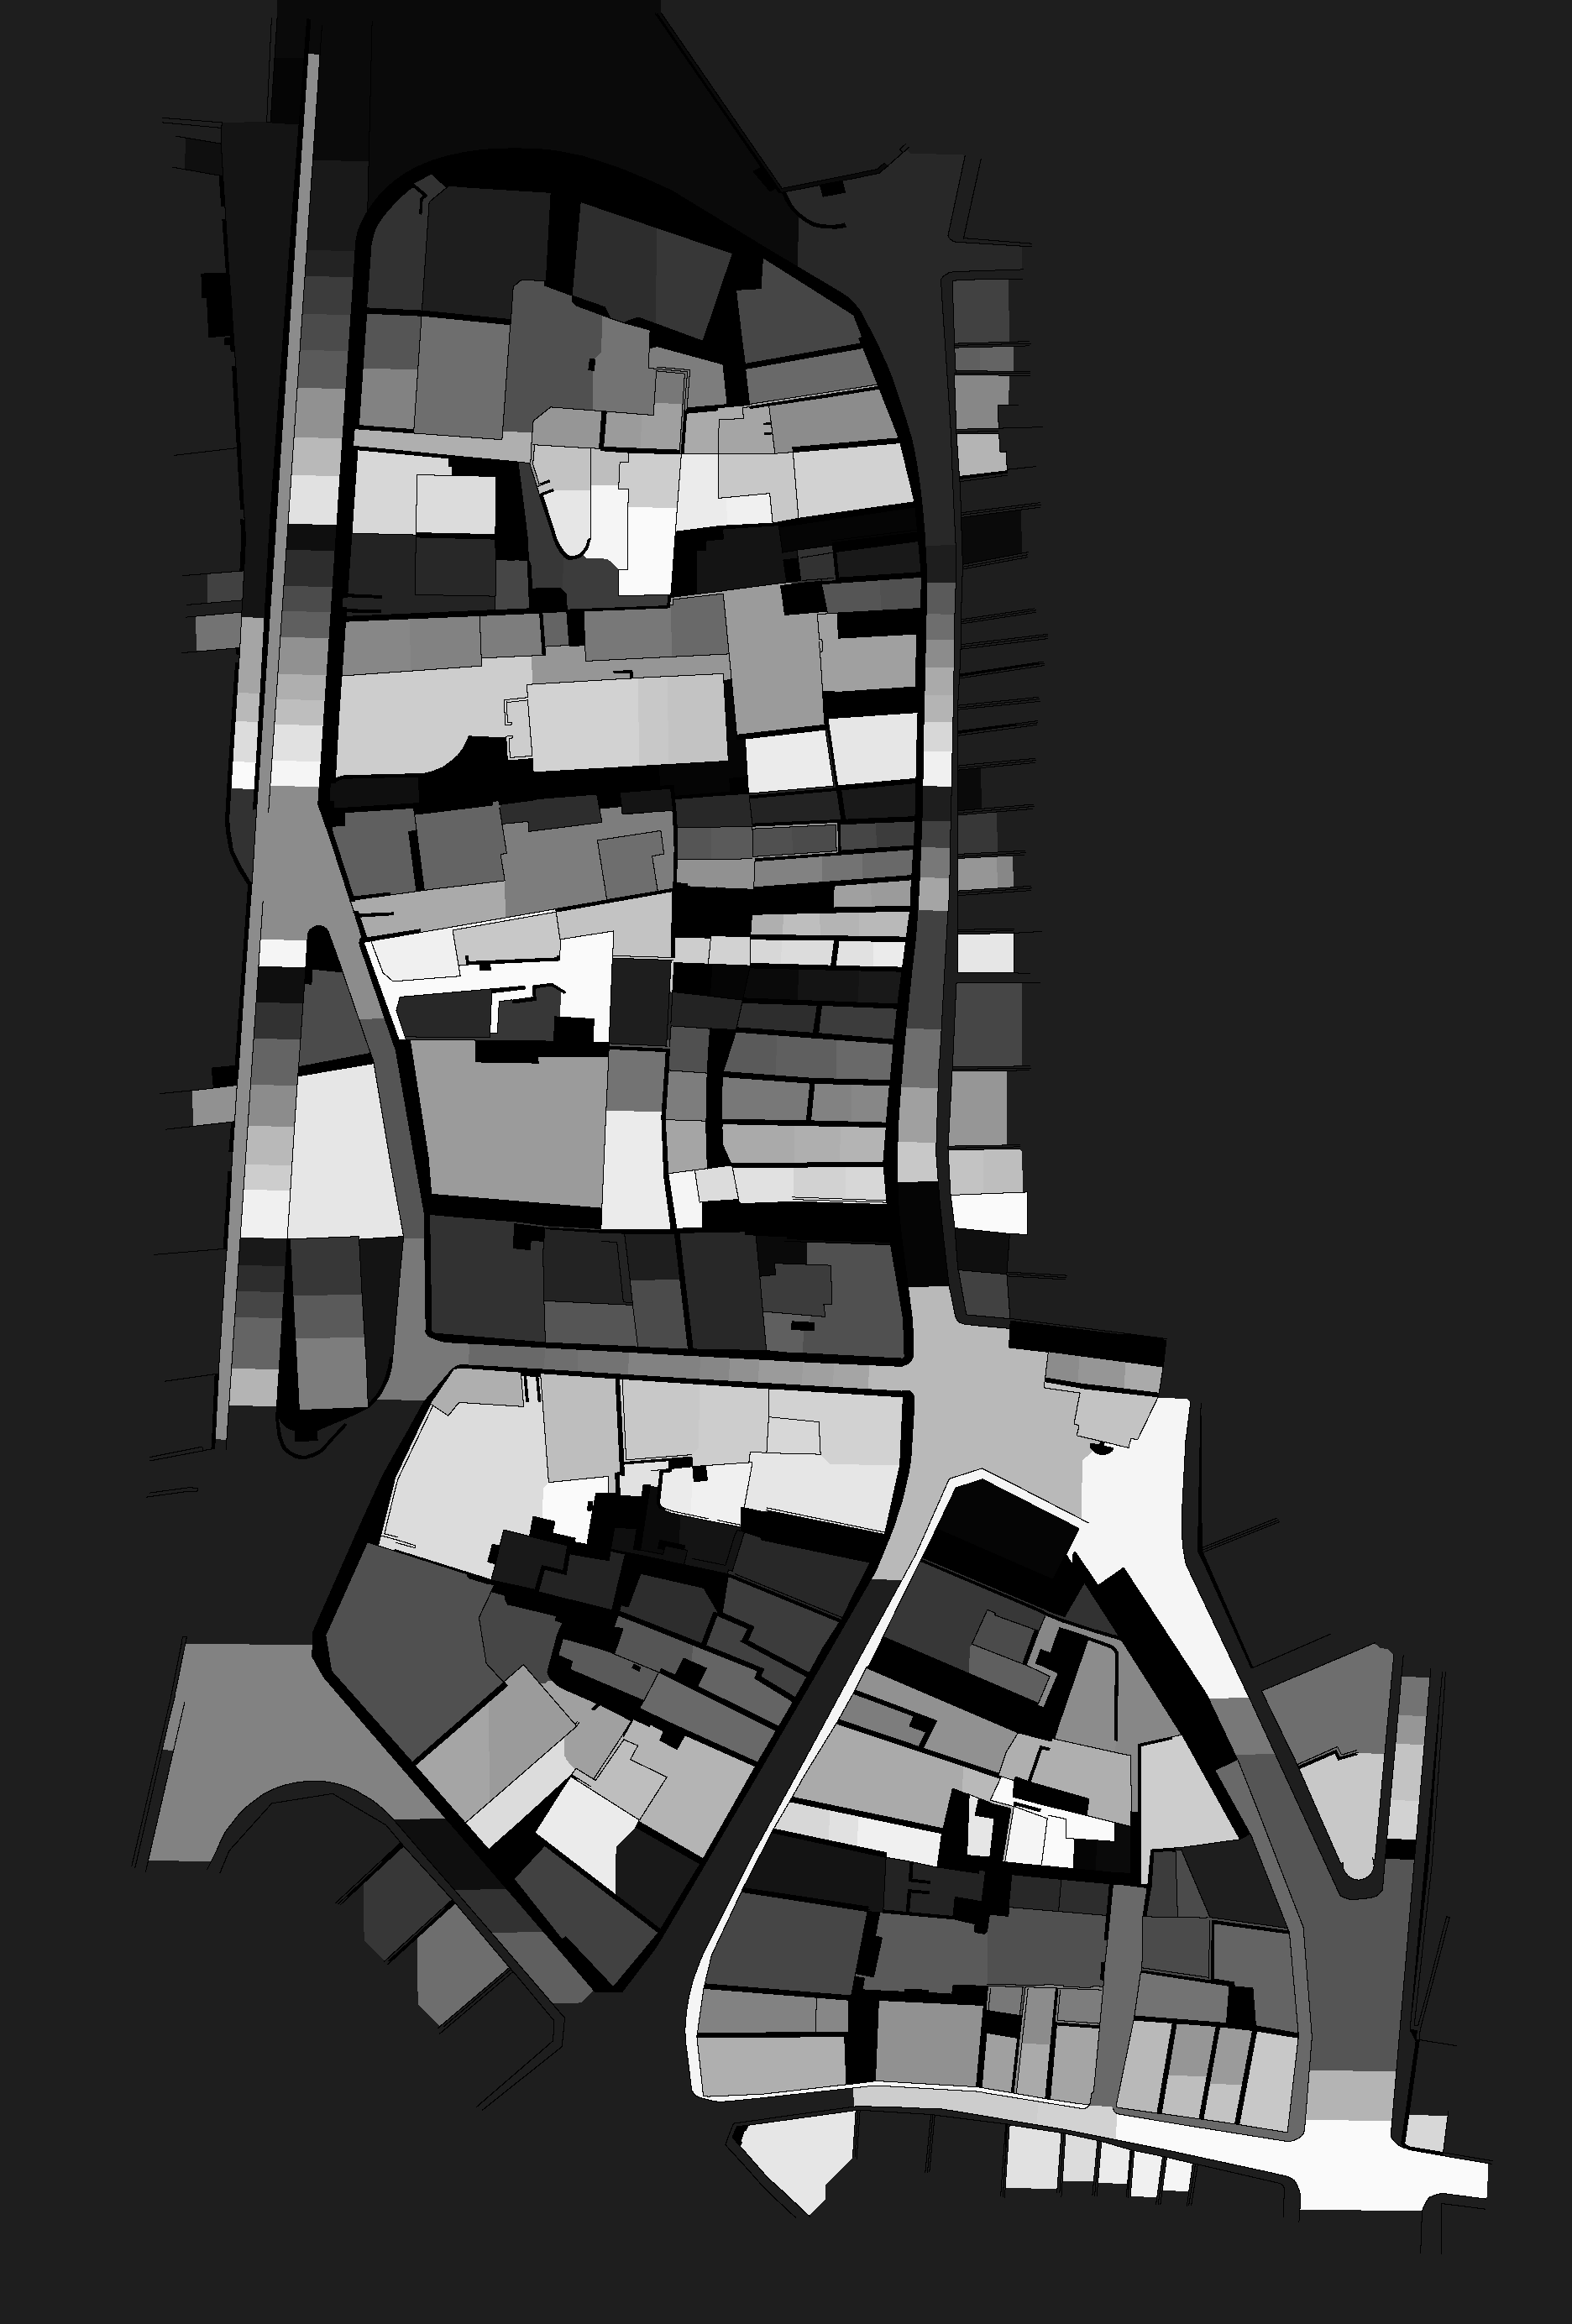
\includegraphics[width=1\linewidth]{images/polygon_recovery/watershed1_distance30_b356.png}  
	   	\caption{min\_distance=30, \\ 356 polygons}
	\end{subfigure}
	\begin{subfigure}[b]{.3\textwidth}
		% include second image
		\centering
		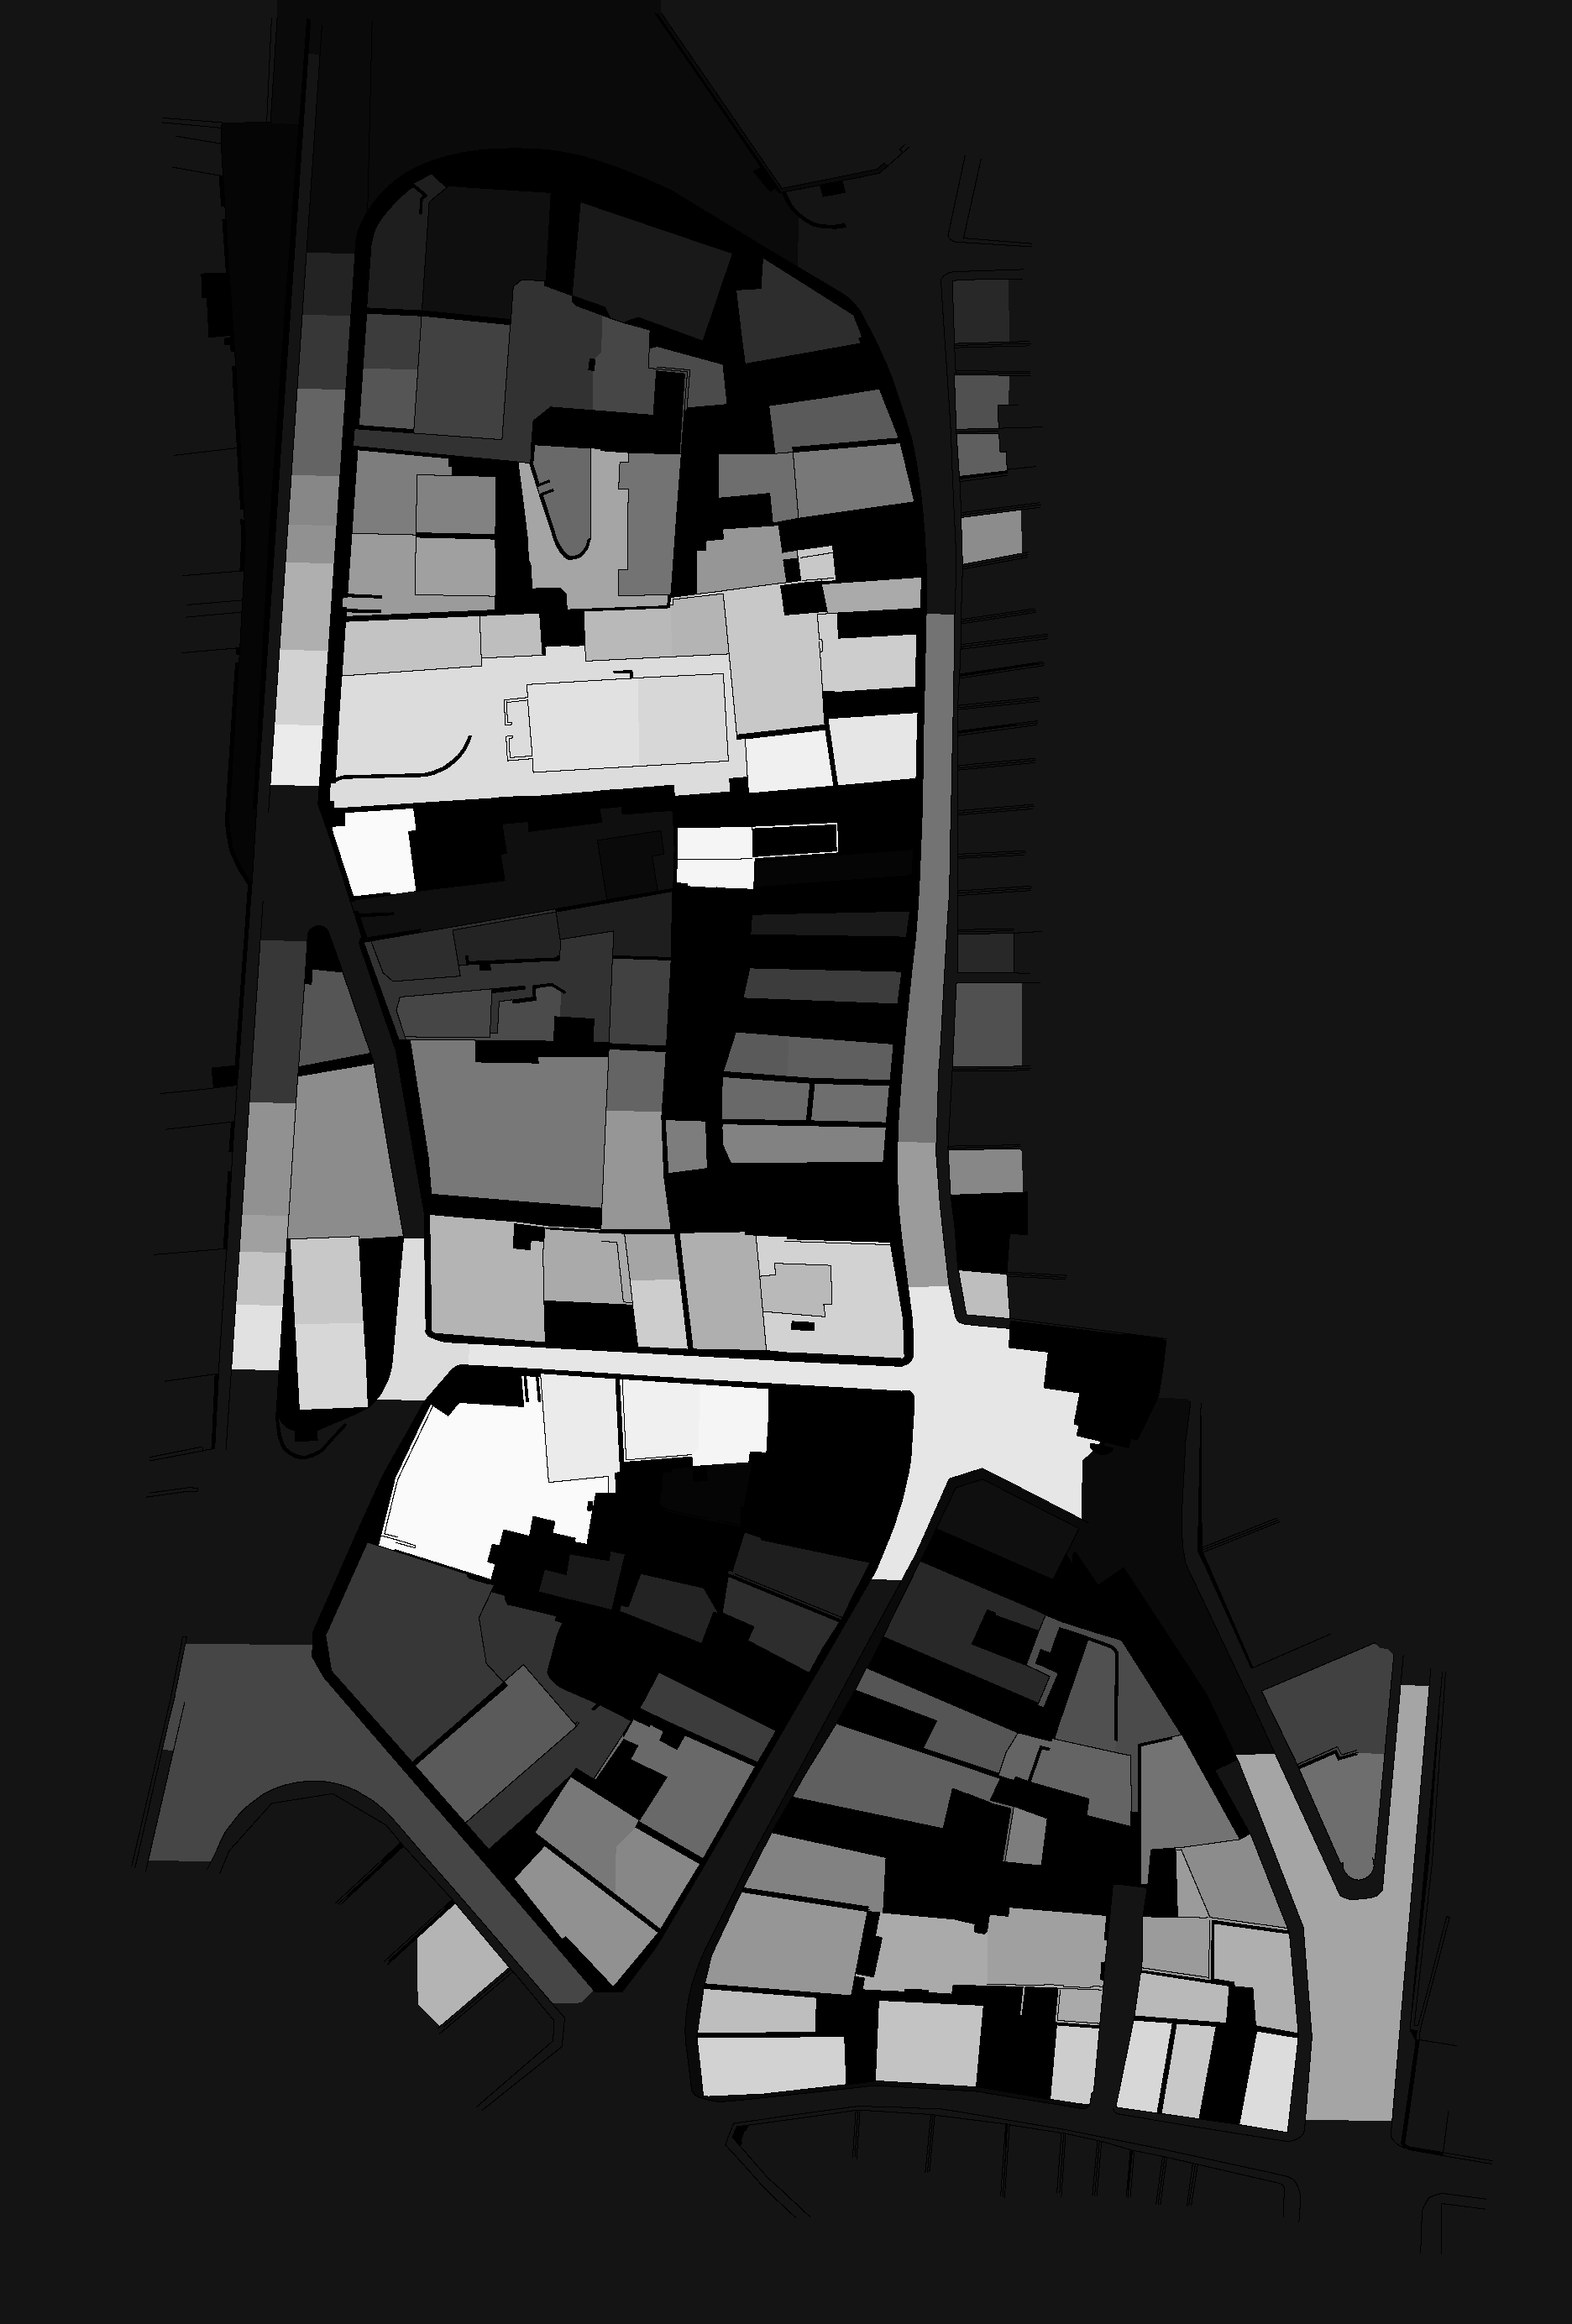
\includegraphics[width=1\linewidth]{images/polygon_recovery/watershed1_distance50_146.png}  
		\caption{min\_distance=50, \\ 146 polygons}
	\end{subfigure}
	
	\rotatebox{90}{\small{~~~~~~~~~~~~~~~~~~~~~~~~~~~~2. Felzenswalb outputs}}
	\begin{subfigure}[b]{.3\textwidth}
		% include first image
		\centering
		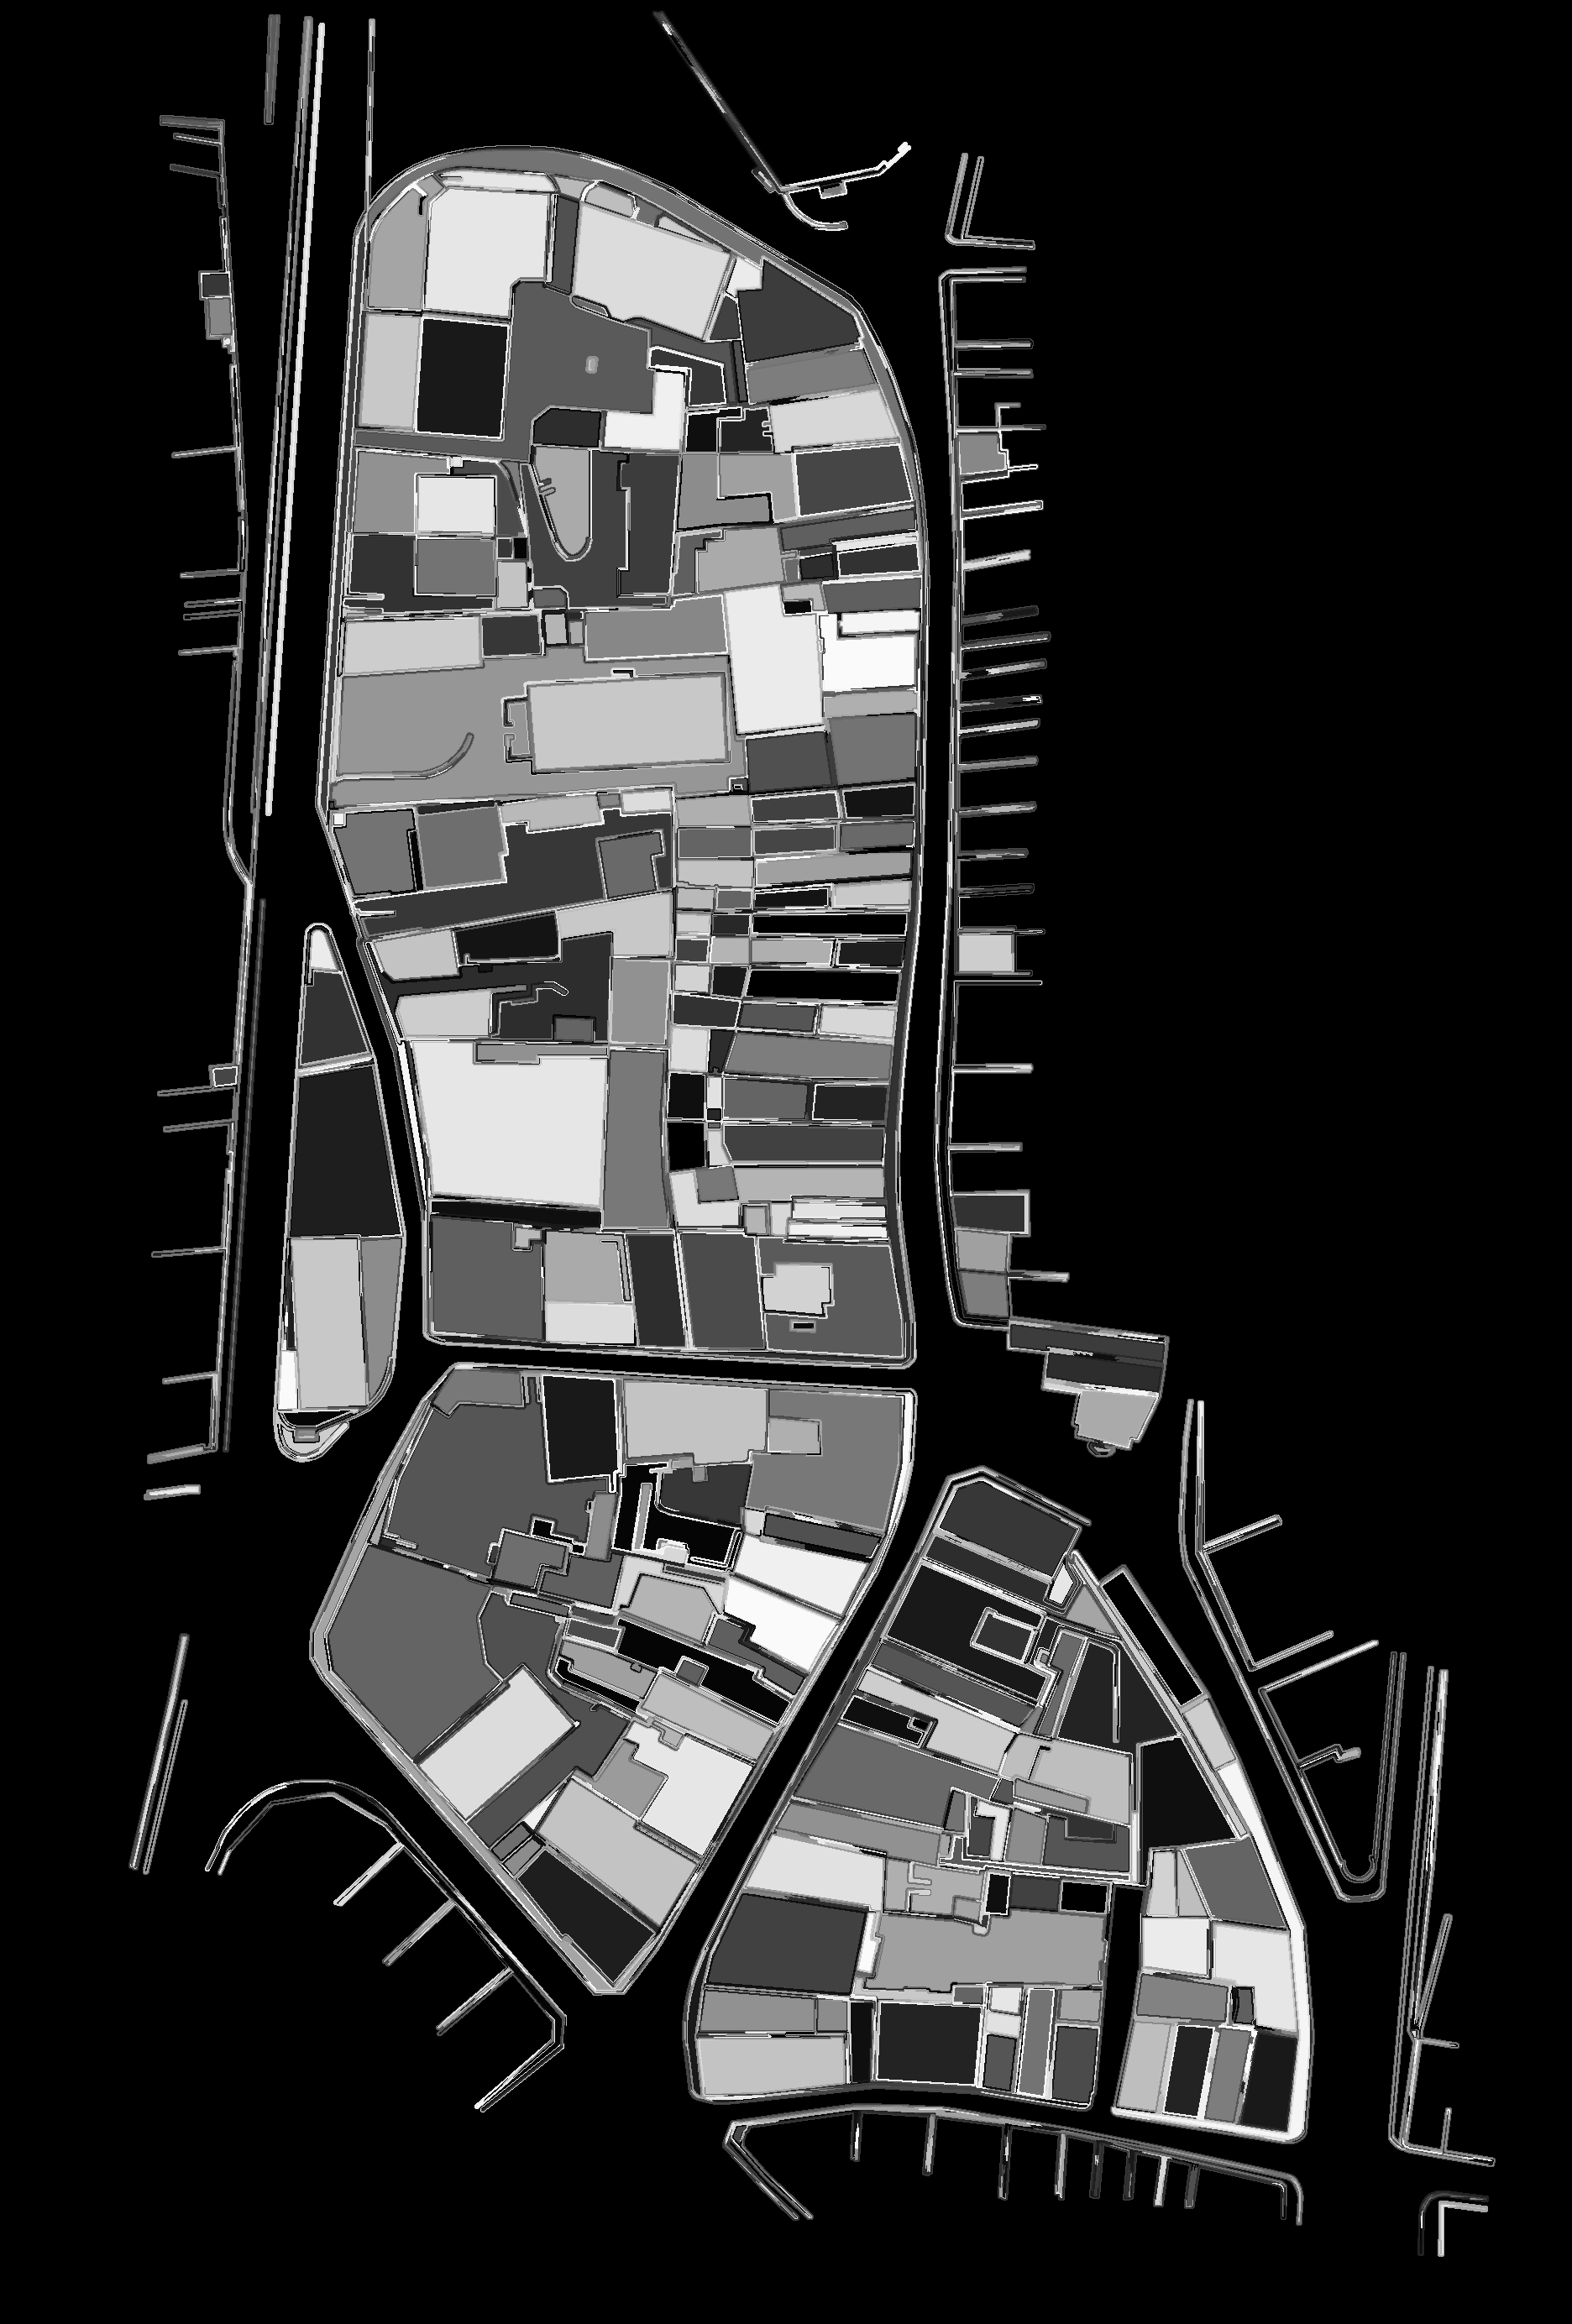
\includegraphics[width=1\linewidth]{images/polygon_recovery/felzenswalb1_scale100_region5511.png}  
		\caption{Observing scale=100, \\ 5511 polygons}
	\end{subfigure}
	\begin{subfigure}[b]{.3\textwidth}
		% include second image
		\centering
		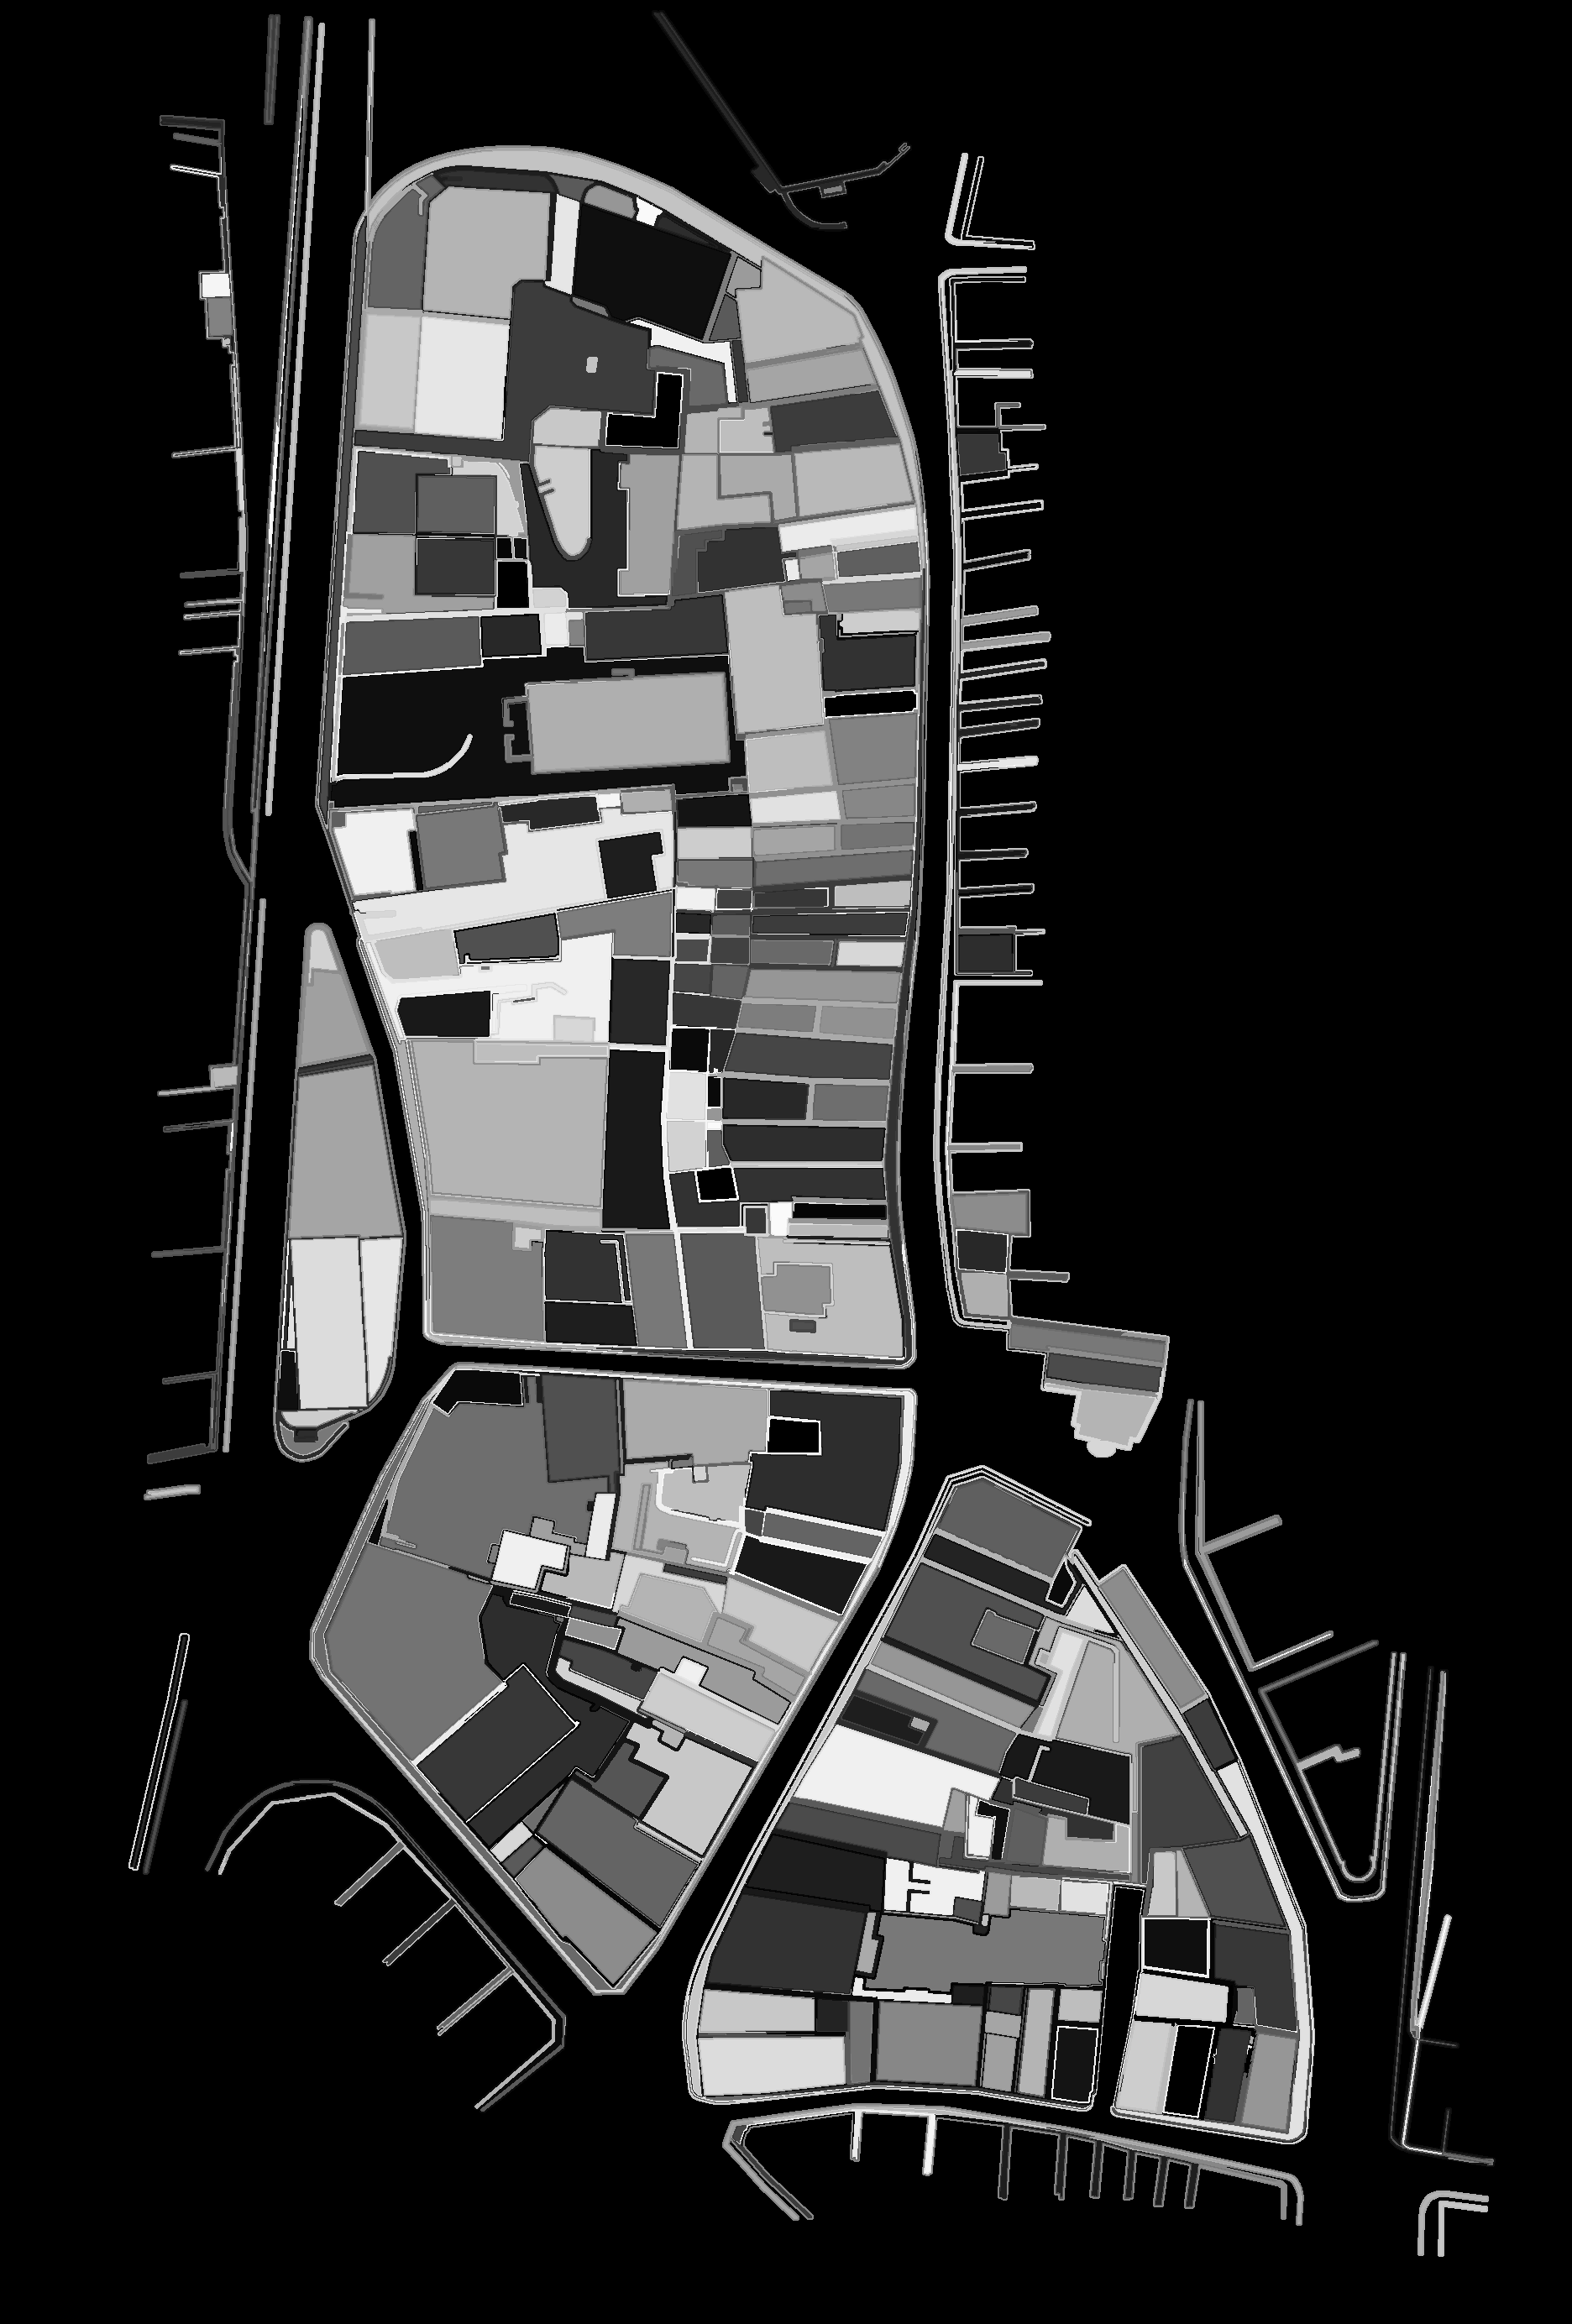
\includegraphics[width=1\linewidth]{images/polygon_recovery/felzenswalb1_scale1000_region1499.png}  
	   	\caption{Observing scale=1000, \\ 1499 polygons}
	\end{subfigure}
	\begin{subfigure}[b]{.3\textwidth}
		% include second image
		\centering
		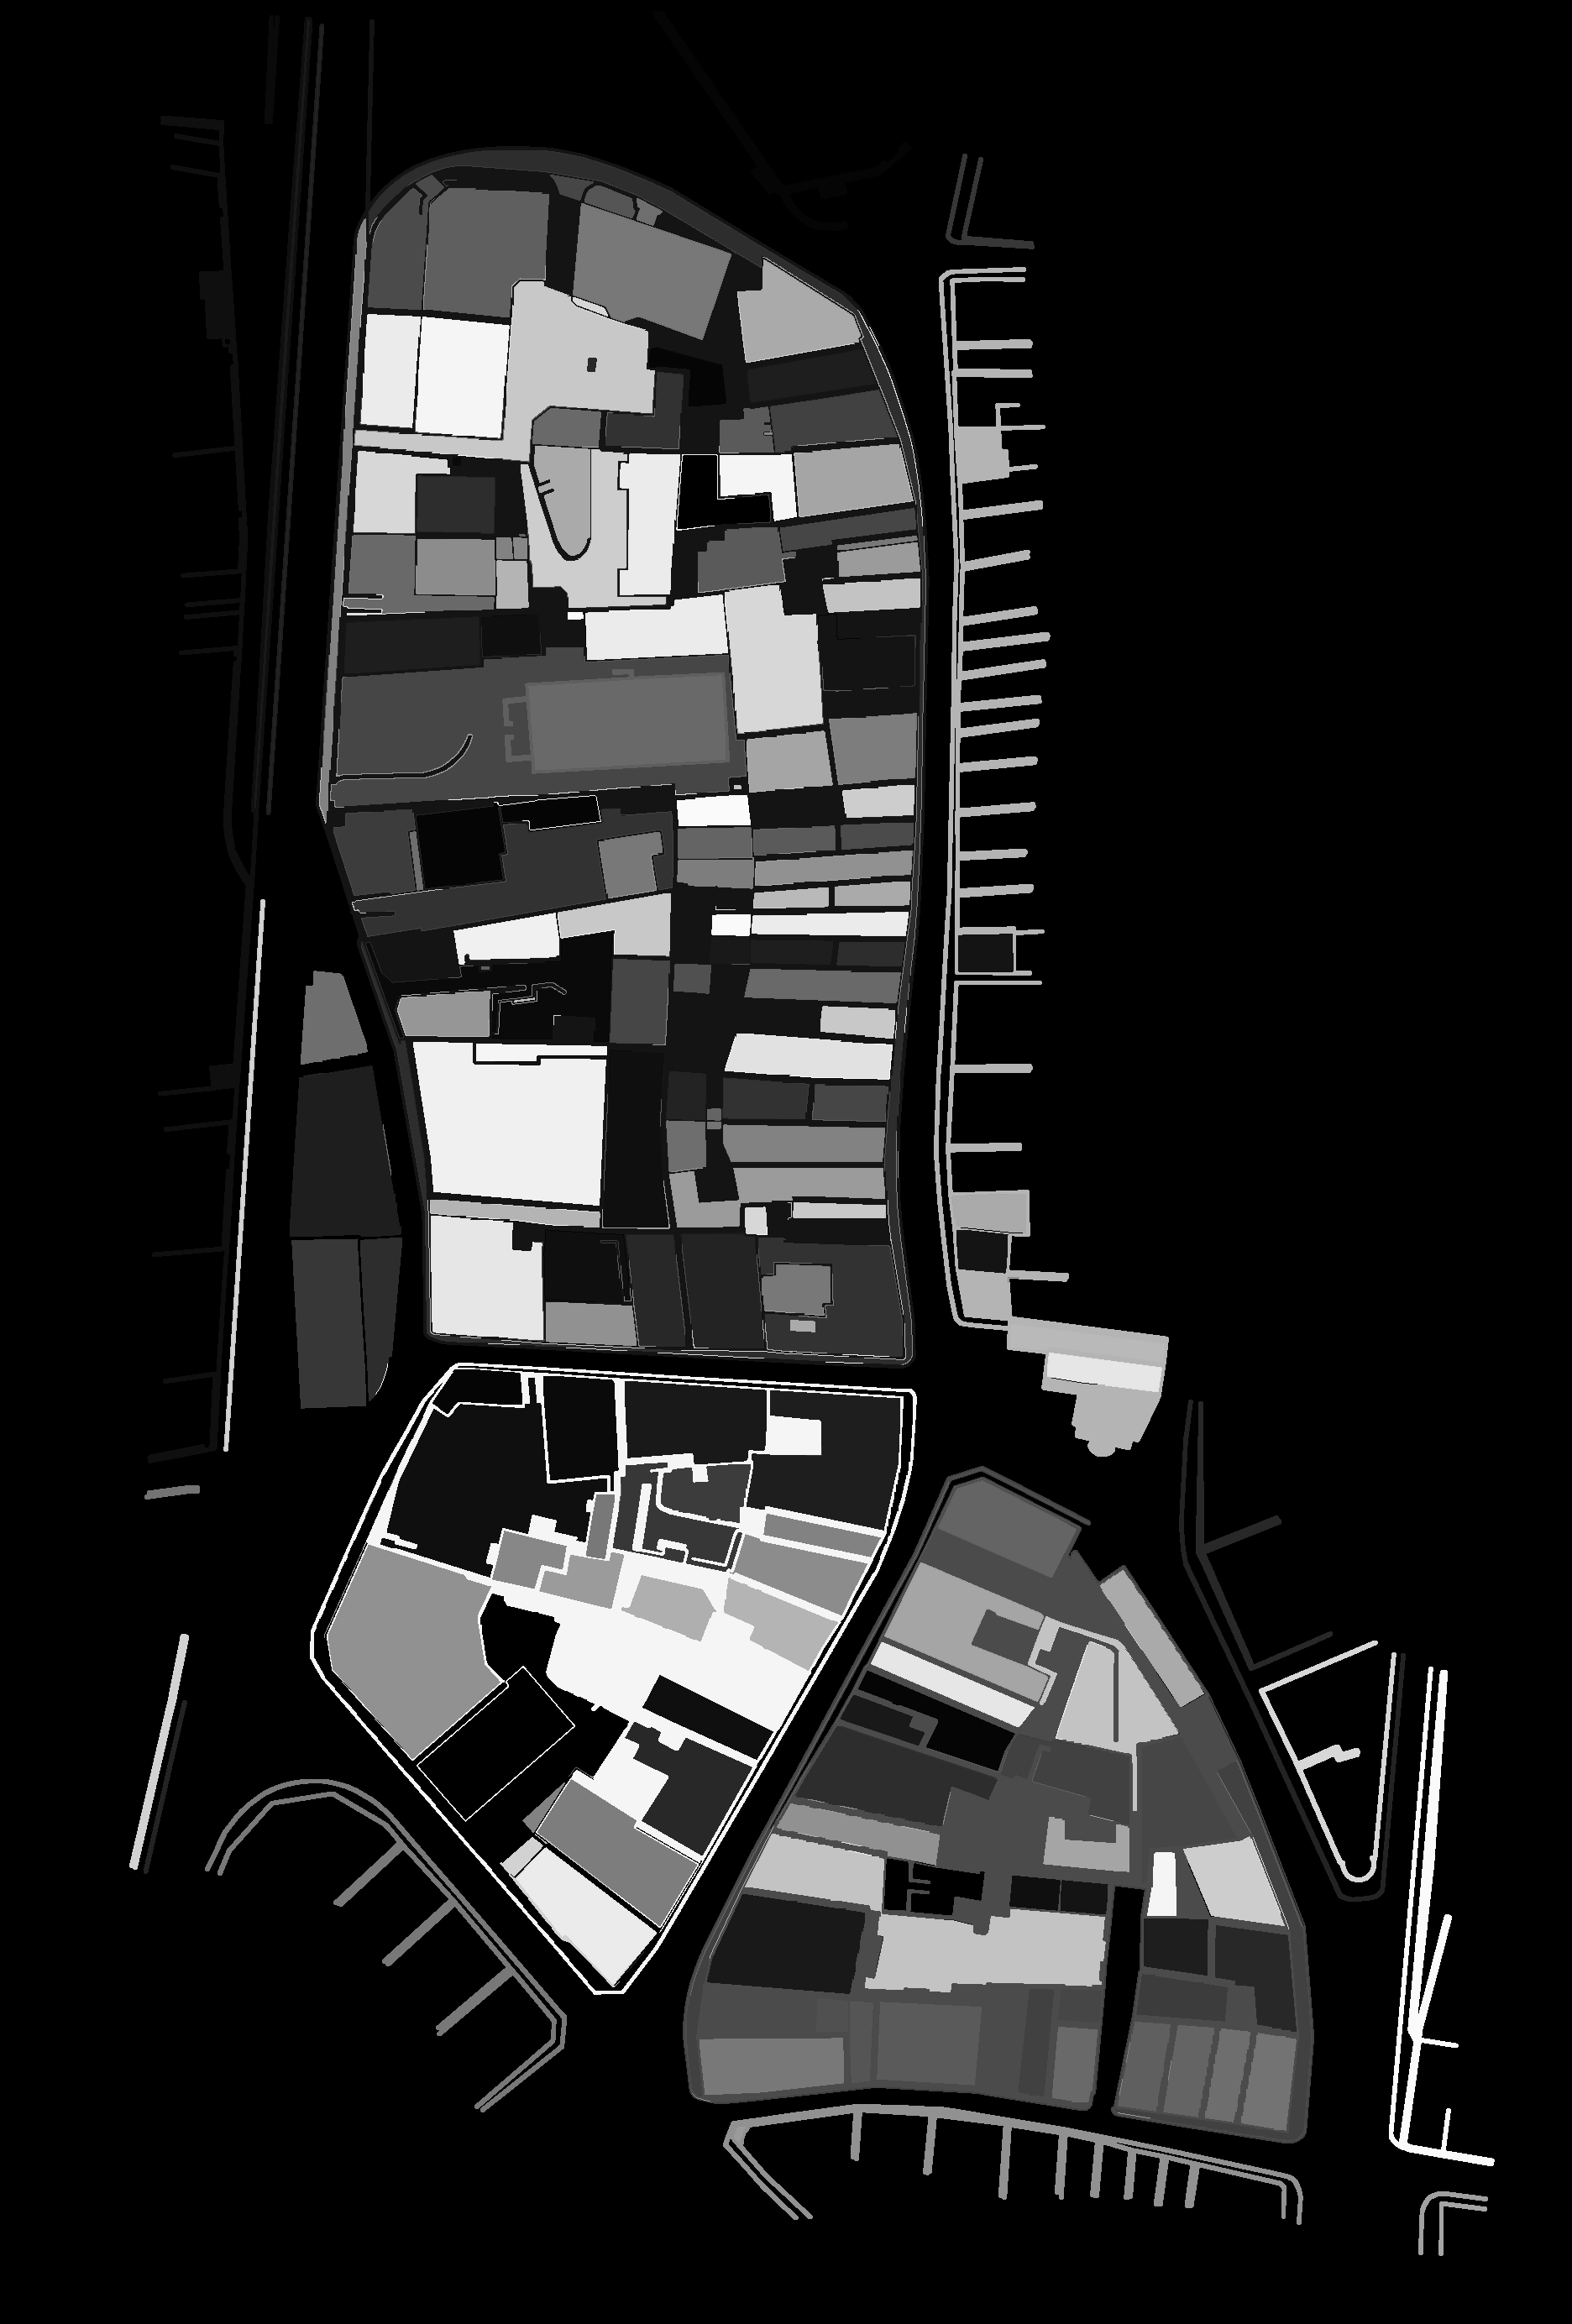
\includegraphics[width=1\linewidth]{images/polygon_recovery/felzenswalb1_scale10000_region543.png}  
		\caption{Observing scale=10000, \\ 543 polygons}
	\end{subfigure}
	
	\caption{Polygon recovery results of Watershed and Felzenswalb algorithm}
	\label{fig:watershed1}
\end{figure}

\begin{figure}[H]
    \centering
	\begin{subfigure}[b]{.3\textwidth}
		% include first image
		\centering
		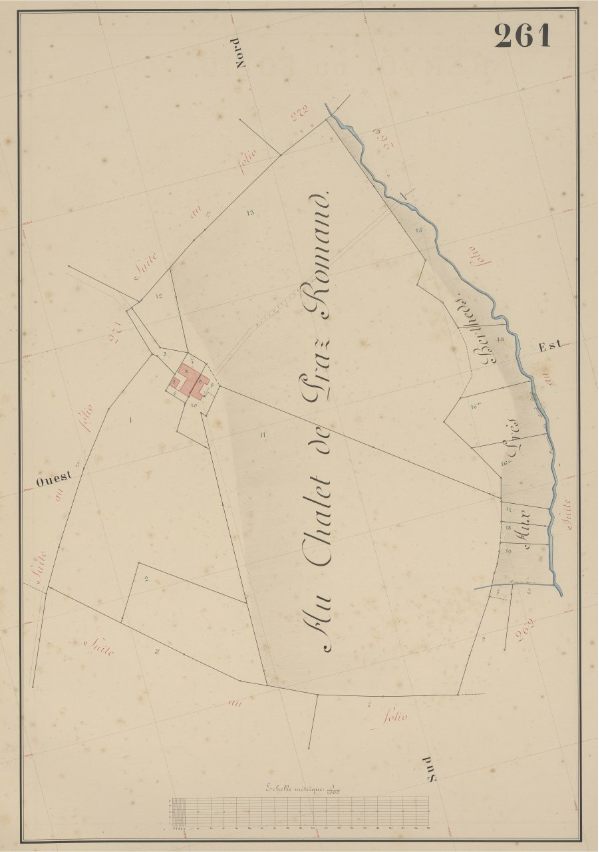
\includegraphics[width=1\linewidth]{images/img5.png}  
		\caption{Original image}
	\end{subfigure}
	\begin{subfigure}[b]{.3\textwidth}
		% include second image
		\centering
		\includegraphics[width=1\linewidth]{images/label5.png}  
		\caption{CNN Prediction outputs}
	\end{subfigure}
	
	\rotatebox{90}{\small{~~~~~~~~~~~~~~~~~~~~~~~~~~~~~~1. Watershed outputs}}
	\begin{subfigure}[b]{.3\textwidth}
		% include first image
		\centering
		\includegraphics[width=1\linewidth]{images/polygon_recovery/watershed2_distance5_b419.png}  
		\caption{min\_distance=5, \\ 419 basins}
	\end{subfigure}
	\begin{subfigure}[b]{.3\textwidth}
		% include second image
		\centering
		\includegraphics[width=1\linewidth]{images/polygon_recovery/watershed2_distance10_b98.png}  
	   	\caption{min\_distance=10, \\ 98 basins.}
	\end{subfigure}
	\begin{subfigure}[b]{.3\textwidth}
		% include second image
		\centering
		\includegraphics[width=1\linewidth]{images/polygon_recovery/watershed2_distance20_b28.png}  
		\caption{min\_distance=20, \\ 28 basins.}
	\end{subfigure}
	
	\rotatebox{90}{\small{~~~~~~~~~~~~~~~~~~~~~~~~~~~~~~2. Felzenswalb outputs}}
	\begin{subfigure}[b]{.3\textwidth}
		% include first image
		\centering
		\includegraphics[width=1\linewidth]{images/polygon_recovery/felzenswalb2_scale100_region961.png}  
		\caption{Observing scale=100, \\ 419 polygons}
	\end{subfigure}
	\begin{subfigure}[b]{.3\textwidth}
		% include second image
		\centering
		\includegraphics[width=1\linewidth]{images/polygon_recovery/felzenswalb2_scale1000_region240.png}  
	   	\caption{Observing scale=1000, \\ 98 polygons}
	\end{subfigure}
	\begin{subfigure}[b]{.3\textwidth}
		% include second image
		\centering
		\includegraphics[width=1\linewidth]{images/polygon_recovery/felzenswalb2_scale10000_region49.png}  
		\caption{Observing scale=10000, \\ 28 polygons}
	\end{subfigure}
	
	\caption{Polygon recovery results of Watershed and Felzenswalb algorithm}
	\label{fig:watershed2}
\end{figure}




\section{Discussion}
The result of the project shows that automatic vectorization of cadastre is feasible through processes: 1) annotation 2) semantic segmentation 3) polygon recovery. With this pipeline, a lot of labor costs and time costs can be saved. 

For the map annotation part, the rule of annotating is not clear, and different people may have different judgment criteria and thus will produce different annotation results, which may result in different semantic segmentation and vectorization outputs. When the dataset is too large, sometimes we have to let more people do the annotation task. In this situation it would be better to have a full discussion about the rules of labeling the objects, It would be a good idea to first annotate one of the maps for everyone, and then they can try to reach a consensus on every annotating detail. With consistent rules, they can make the dataset with higher quality and accuracy to fit their goal. 

Regarding the semantic segmentation performance, UNet architecture with ResNet101 as the encoder shows a good ability to solve the cadastre map segmentation problem, and the vast majority of "edges" are well-predicted with high quality (MIoU=0.9018, IoU of "edge"=0.808, Precision of "edge"=0.8816, Recall of "edge"=0.9063). We also randomly chose additional 12 maps from the cadastre without annotating and training for the model to predict. After "patching-predicting-reconstituting" processes, the prediction outputs have shown great inference to all of these additional 12 maps, which indicate that the model performed strong robustness for the whole cadastre dataset. But we also found that the model performs unsatisfactorily in the situation where prediction objects are overlapped with text descriptions. We have to admit that those overlapped texts indeed interfere with the prediction results, but we could try to adjust the detail of the model structure or dataset processing method to better solve this problem. For example, we can consciously add patches containing the overlapping problem in the dataset to improve the ability of the model to handle this situation. Also, we can try to change the data augmentation method and add more image transformations like gamma transformation, Gaussian blur, etc to strengthen the robustness of the model. 

Both watershed transformation and the Felzenswalb algorithm have shown acceptable results for polygon recovery, but both of these algorithms have some common limitations. Firstly, both of them have a key parameter to set by us, which relies more on our experience (minimum catchment basin distance for watershed transformation, observation scale for Felzenswalb), and it is hard to quickly set a suitable parameter to segment polygons of the map. Secondly, different maps have different suitable parameters. if we use either of the two algorithms when processing the whole cadastre with more than 300 maps, maybe we have to manually adjust the algorithm parameter for each map to get a great polygon recovery result, and this will cost a lot of time for researchers and could not meet our final goal of "automatic vectorization" and because the limiting time, we do not have enough time to deep in this domain. Since these parameters have a relationship with the dense of the map boundaries, the denser the map: the bigger the parameter (minimum distance for the watershed, observing scale for Felzenswalb should be set), in the future it is possible to explore methods to automatically choose the key parameters of these algorithms to suit the majority of the maps to save time for researchers. And more polygon recovering algorithms should be experimented with to find a better method to segment polygons in cadastre maps.

Finally, we think that to achieve the automatic vectorization goal, we need to manually label the polygon recovery outputs with particular software to get the vector image like the "shapefile (.shp)" format for example.  But maybe there exist methods to automatically transfer polygon recovery output or CNN prediction results to the vector image result. In the future, maybe we can try to make use of the contour finding algorithm provided in the "scikit-image" library to achieve this process, and thus we can eventually achieve the automatic vectorization goal: automatically get the vector image for the original cadastre map.


\newpage








\clearpage
\bibliography{biblio.bib}
\bibliographystyle{plain}    % author-year citation style
% \bibliographystyle{siam}  % numbered citation style (deprecated by some)

\end{document}

